%%%%%%%%%%%%%%%%%%%%%%%%%%%%%%%%%%%%%%%%%%%%%%%%%%%%%%
%% Fleet dynamics models in FLBEIA
%%%%%%%%%%%%%%%%%%%%%%%%%%%%%%%%%%%%%%%%%%%%%%%%%%%%%%

\documentclass[12pt, halfline, a4paper]{ouparticle}

\usepackage[utf8]{inputenc}
\usepackage{lscape}
\usepackage{rotating}
\usepackage{booktabs}
\usepackage{longtable}
\usepackage{subfigure}
\usepackage{natbib}
\usepackage{xcolor}
\usepackage{listings}

%% For embedding R code
\lstset{language=R,
basicstyle=\footnotesize,
breaklines=true,
backgroundcolor=\color{aliceblue},
keywordstyle=\color{blue},
commentstyle=\color{darkgreen},
stringstyle=\color{purple}}

\definecolor{aliceblue}{rgb}{0.94,0.97,1.0}
\definecolor{darkgreen}{rgb}{0.0, 0.2, 0.13}

%%%%%%%%%%%%%%%%%%%%%%%%%%%%%%%%%%%%
\begin{document}

\title{Working title: Alternative hypothesis for location choice in
	mixed-fishery management strategy evaluation}

\author{
	\name{Paul J. Dolder}
	\address{GMIT}
	\email{paul.dolder@research.gmit.ie}
	\address{CEFAS}
	\email{paul.dolder@cefas.co.uk\thanks{Corresponding author} }
	\and
	\name{Cóilín Minto}
	\address{GMIT}
	\email{coilin.minto@gmit.ie}
	\and
	\name{Dorleta Garcia}
	\address{AZTI}
	\email{dgarcia@azti.es}
}

\abstract{Some text here}

\date{\today}

\keywords{MSE, mixed fisheries, fleet dynamics, RUM, Markov}

\maketitle

\section{Introduction}
\label{intro}

Most fisheries worldwide are mixed. Evaluation of management performance is
still based on single-species, failing to take account of fleet dynamics;
technical (mixed-fishery) interactions affect the outcome of management
measures through either discarding unwanted catch or ``choking" of quota when
first limit reached. It's important for MSEs to take account of these
interactions when evaluating management strategies in order to move towards a
more holistic approach to fisheries management.  \\

In order to address this mixed fishery methods have been developed and applied
to numerous case studies (REFs). The mixed-fishery approach models activity of
fleets (vessels of similar physical characteristic) and how the deployment of
fishing effort in different métier (activity defined by similar catch patterns)
contribute to catch of multiple stocks simultaneously. The assumption about the
amount of fishing effort deployed in each of the métier and stability of
catchability for the different stocks determines the outcome for the fishery in
terms of fishing mortality and catch for each stock. The sum of the different
fleets activity (and their catch composition and selectivity) thus provides a
different picture on exploitation of stocks exploited concurrently. \\ 

A limitation in evaluated management strategies from a mixed fishery
perspective is the lack of operating model to account for how fisher behaviour
affects catch of multiple stocks. Location choice is one key decision that
effects catch in mixed fisheries. Different locations have different density of
target and non-target species, therefore choice of where to fish determines how
much of each species caught. This is rarely taken into account in simulations
of management strategies.\\

Here, we extend application of FLBEIA to include commonly used fleet dynamics
models for location choice. This includes the Caddy Gravity model, the
conditional logit Random Utility model and a Markov transition model. We apply
the models to the Celtic Sea demersal fisheries, with location choice for Irish
otter trawlers among nine areas determined by each of the location choice
models and compared to a base case of constant effort. In doing so we show how
different outcomes may be achieved given different assumptions about location
choice. We recommend implementation of different fleet location choice
operating models when undertaking mixed-fishery MSEs in order to incorporate
this important dynamic alongside plausible biological dynamics to better
characterise outcomes for fisheries indicators. \\

FLBEIA \citep{Garcia2017} is a bioeconomic framework for simulating management
strategies for multi-stock multi-fleet fisheries taking account of
mixed-fishery (technical) interactions. It is based on the FLR library of
fisheries management tools \citep{Kell2007}, and can be used to evaluate the
effect of different harvest rules and model selectivity improvements and
spatial closures to assess their impact on biological and economic components
of the stocks and fisheries.  FLBEIA takes a modular approach, with components
for biological and fleet operating models and a management procedure taking
account of the perceived state of the system and implementation of defined
management rules, thus taking account of full feedback and uncertainty in
management outcome (See Figure \ref{fig:flbeia}). \\

Applications typically assume constant share of a fleets fishing effort among
different métier \citep{Ulrich2016, Garcia2020}, with exploitation per unit of
effort for different fleets remaining static inter-annually. This limits
understanding of the impact of fleet dynamics on outcomes for different
fisheries strategies. 

\section{Methods}
\label{meth}

We implemented five location choice models within the FLBEIA modelling
framework: a base model where effort remains the same as in the past, a gravity
model, a hybrid gravity and base model, a conditional logit Random Utility
Model (RUM) and a Markov transition model. Each of the models were fit to data
and effort was dynamically predicted within the simulation, with predictions of
effort updated based on the development of the fishery dynamics.  \\

We applied the models to the Irish Otter trawl fleet in selecting among 9
different locations (defined as métier) fishing in the Celtic Sea (ICES
subdivisions 7bc,e-k), including following closure of one of the métier. We
then compared the outcomes for the fisheries in terms of catch for the fleet
and stock-based fishery indicators to assess the differences in outcome given
the location choice model used.

\subsection{FLBEIA}

To model inter-annual fleet dynamics, FLBEIA explicitly defines the
relationships between the fishing effort of each fleet, the allocation of that
effort among different métier, the catchability for the métier for each stock
and the catch \citep{Garcia2017a}. Such that:

\begin{equation}
 C_{f,s} = q_{f,m,s}\cdot B_{s}^{\beta_{f,m,s}} \cdot \left(E_{f}\cdot
	 \delta_{f,m} \right)^{\alpha_{f,m,s}}	
\end{equation}

Where $C_{f,s}$ is the catch of fleet $f$ for stock $s$, $q$ is the
catchability for métier $m$ and $B$ biomass for the stock, with $E_{f}\cdot
\delta_{f,m}$ the Effort $E$ and $\delta$ the métier effort share (0..1).
$\alpha$ and $\beta$ are Cobb-Douglas production coefficients, where when equal
to 1 gives a linear relationship between fishing effort and catch for a given
biomass. For simplicity, the age subscript has been dropped but the equation
also applies on an age-by-age basis. \\

The overall effort deployed by the fleet determines the catch of each stock. An
assumption must be made as to how much effort a fleet deploys in response to
the available fishing opportunities. Options include stopping fishing when the
first quota is reached (`min'), the last quota is reached (`max') or a spectrum
in between for each of the available stocks `st': this approach is known within
FLBEIA as `Simple Mixed Fishery Behaviour'.  \\

FLBEIA can be installed directly as a library in R from github
(\url{www.github.com/flr/FLBEIA}).  Full details of setting up an FLBEIA
simulation can be found in the technical manual \citep{Garcia2017a} and
examples (\url{https://flr-project.org/doc/FLBEIA_A_Simple_Example.html}). 

\subsection{Location choice models}

The five models implemented include:\\

(i) A \textbf{base model} (b) where the proportion of effort in métier $m$ at time
$t$ is:
\begin{equation}
p^{b}_{m,t} = \overline{p}_{m}
\end{equation}

(ii) A \textbf{Gravity model} (g) where the proportion of effort in métier $m$ at
time $t$ is given by: 
\begin{equation}
p^{g}_{m,t} = \frac{\overline{R}_{m}}{\sum\limits_{m=1}^{M}\overline{R}_{m}} 
\end{equation}

where $\overline{R}_m$ is the expected revenue per unit effort in a given
métier, where $R$ for a given year is defined as: 
\begin{equation}
R_{m,t} =  \sum\limits_{s=1}^{S} L_{m,t,s} P\text{x}_{s} 
\label{eqn:ppue}
\end{equation}

comprised of the sum of the landings $L$ of each species $s$ for métier $m$ at
time $t$ multiplied by the price $P\text{x}_{s}$. It's also possible to
implement this approach based on profit per unit effort, where the cost per
unit of effort of fishing in a particular métier are subtracted from equation
\ref{eqn:ppue}. \\

(iii) A \textbf{Gravity and Past Share Combination}, an alternative formulation
of a gravity model was included, where 80\% (denoted by $\alpha$) of the effort
allocation was determined by past effort (tradition, or inertia) and 20\% by
the gravity model (economic opportunism). This Gravity-Tradition combination
model (superscripted $c$) is given by:
\begin{equation}
	p^{c}_{m,t} = \alpha \cdot p^{p}_{m,t} + (1 - \alpha) \cdot p^{g}_{m,t}
\end{equation}
where $\alpha$ controls the proportional weighting of either model. \\ 

(iv) A \textbf{Random Utility Model} where a case- and choice- specific
multinomial logit RUM ($r$) is implemented so that:  
\begin{equation}
p^{r}_{m,t} = \frac{e^{\beta_{m} \cdot X_{t} + \gamma \cdot Z_{m,t}}}{1 + 
	e^{\beta_{m} \cdot X_{t} + \gamma \cdot Z_{m,t}}}
\label{eqn:rum}
\end{equation} 

The choice-specific covariates $Z_{m,t}$ can comprise catch rates or revenue
from stocks from fishing in the métier, while the case-specific covariates
($X_{t}$ included a seasonal effect. \\

(v) A \textbf{Markov transition model} where the proportion of effort in métier
$m$ at time $t$ is the sum of the transitioned proportions of effort from areas
$z$ (departing area) at time $t-1$:
\begin{equation}
p^m_{m,t} = \sum_{z = 1}^{M} p^m_{z, t-1} p^m_{z,m,t}
\end{equation}

where the transition probabilities are given by the logit function:

\begin{equation}
p^m_{z,m,t} = \frac{e^{\beta_{z,m} X_{t}}}{1+e^{\beta_{z,m} X_{t}}}
\end{equation}

Seasonal changes can be included through the effect of month in the vector
$X_t$. 

\subsection{Location choice model specification in FLBEIA}

Each of the models has been implemented flexibly so that the covariates can be
derived from any of the stocks catch rates or elements from an internal FLBEIA
object. For example, by specifying a particular stock or slot from an
FLMetierExt (e.g. effshare) it can be included in the model estimation and
prediction of effort allocation. \\

Here we only specify the changes required to implement the location choice
models in FLBEIA; the general model setup is described in \cite{Garcia2017a}
and will be specific to case studies. Each of the location choice models can be
implemented directly in FLBEIA through the following changes (note i is the
base case, so no changes are needed to the standard set up to implement this
approach): \\

For all models, the effort.model should be set an SMFB\_ES (Simple Mixed
Fishery Behaviour Effort Share) within the fleets\_ctrl object passed to the
main FLBEIA function. This accesses the location choice model settings:

\begin{lstlisting}[language=R]
fleets.ctrl[[fleet]][['effort.model']]   <- 'SMFB_ES'
\end{lstlisting}

(ii) \textbf{Gravity model} \\

To implement the gravity model requires no model formula to be passed to
FLBEIA, but you can set different options once the effort share model has been
set. The following implements a gravity model based only on the revenue from
each of the métier:

\begin{lstlisting}[language=R]
fleets.ctrl[[fleet]][['effshare.model']] <- 'gravity.flbeia'
fleets.ctrl[[fleet]][['gravity.model']] <- 'revenue' ## alternative:profit 
\end{lstlisting}

(iii) \textbf{Gravity tradition model} \\

To implement the gravity-tradition hybrid model requires an additional option
to be passed to FLBEIA specifying the proportion of the métiers effort that
should be determined by the past share, or tradition:

\begin{lstlisting}[language=R]
fleets.ctrl[[fleet]][["gravity.tradition"]] <- 0.8 ## 80 % from tradition
\end{lstlisting}

(iv) \textbf{Random Utility Model} \\

To implement a RUM, the model must first be estimated using the R package
\textit{mlogit} \citep{Croissant2019} and the function \textbf{mlogit}.
Following estimation, the model object should be passed to FLBEIA as follows:

\begin{lstlisting}[language=R]
fleets.ctrl[[fleet]][['effshare.model']] <-  'mlogit.flbeia'
fleets.ctrl[[fleet]][['mlogit.model']]   <-  RUM_model_fit
\end{lstlisting}

(v) \textbf{Markov transition model} \\

The Markov model is implemented with the R package \textit{nnet} and the
function \textbf{multinom}. Following estimation, the model object should be
passed to FLBEIA as follows:

\begin{lstlisting}[language=R]
fleets.ctrl[[fleet]][['effshare.model']] <-  'Markov.flbeia'
fleets.ctrl[[fleet]][['Markov.model']]   <-  Markov_fit 
\end{lstlisting}



\subsection{Applied example}

We assume that the Irish Otter trawl fleet stops fishing when the effort
corresponding to the closest stock specific effort in the previous year for all
location choice models. Thus the difference in the location choice model
scenarios was down exclusively to  \\ 



\begin{itemize}
	\item Implementation of fleet dynamics models in FLBEIA (pseudo-code)
	\item Conditioning of seasonal FLBEIA model
		\begin{itemize}
			\item 4 seasons
			\item Metiers defined by spatial patterns in catch
			\item Implement fleet dynamics model for Irish otter
				trawlers
		\end{itemize}
	\item Fitting of models 
		\begin{itemize}
			\item Gravity
			\item Gravity + tradition
			\item RUM
			\item Markov 
			\item Model selection for RUM and Markov.
		\end{itemize}
	\item Simulations including closures
		\begin{itemize}
			\item Close a metier, how does effect reallocate
		\end{itemize}
	\item MSE with different fleet dynamics models as OM
\end{itemize}

\section{Results}
\label{res}

Characteristics of the different modelling approaches. \\

How each model is affecting by different species catch rates \\.

Combining inference from the models (different location choice OM, conclusions
about overall strategy. \\


\section{Discussion}
\label{dis}

\section{Conclusions}
\label{con}


\begin{notes}[Acknowledgements]
The authors would like to thank...
\end{notes}

\bibliographystyle{apalike}
\bibliography{FLBEIA}

\clearpage

\begin{table}
	\center
	\begin{tabular}{p{4cm} p{3cm} p{2cm} p{2cm} p{2cm}}
		\toprule
		Stock & Code & Fmsy & Blim & Bmsytrigger \\
		\hline
		Cod & COD & 0.35 & 7,300  & 10,300 \\
		Haddock & HAD & 0.4 & 6,700 & 10,000 \\
		Anglerfishes & ANF & 0.28 & 16,032 & 22,278 \\
		European Hake & HKE & 0.28 & 32,000 & 45,000 \\
		Megrims & LEZ & 0.191 & 37,100 & 41,800 \\
		Whiting & WHG & 0.52 & 25,000 & 35,000 \\
		\textit{Nephrops} FU16 & NEP16 & 0.062 & 19,880 & 49,700 \\
		\textit{Nephrops} FU17 & NEP17 & 0.085 & 4,637 & 11,593 \\
	        \textit{Nephrops} FU19 & NEP19 & 0.093 & 4,032 & 10,080 \\
		\textit{Nephrops} FU2021 & NEP2021 & 0.06 & 33,040 & 82,600 \\
		\textit{Nephrops} FU22 & NEP22 & 0.128 & 7,585 & 18,963 \\
		\bottomrule
	\end{tabular}
	\label{tab:brp}
	\caption{Biological Reference Points used in the Harvest Control Rules for each
		stock when setting the overall annual Total Allowable Catch.}
\end{table}

\clearpage

\begin{figure}[!ht]
	\centering
	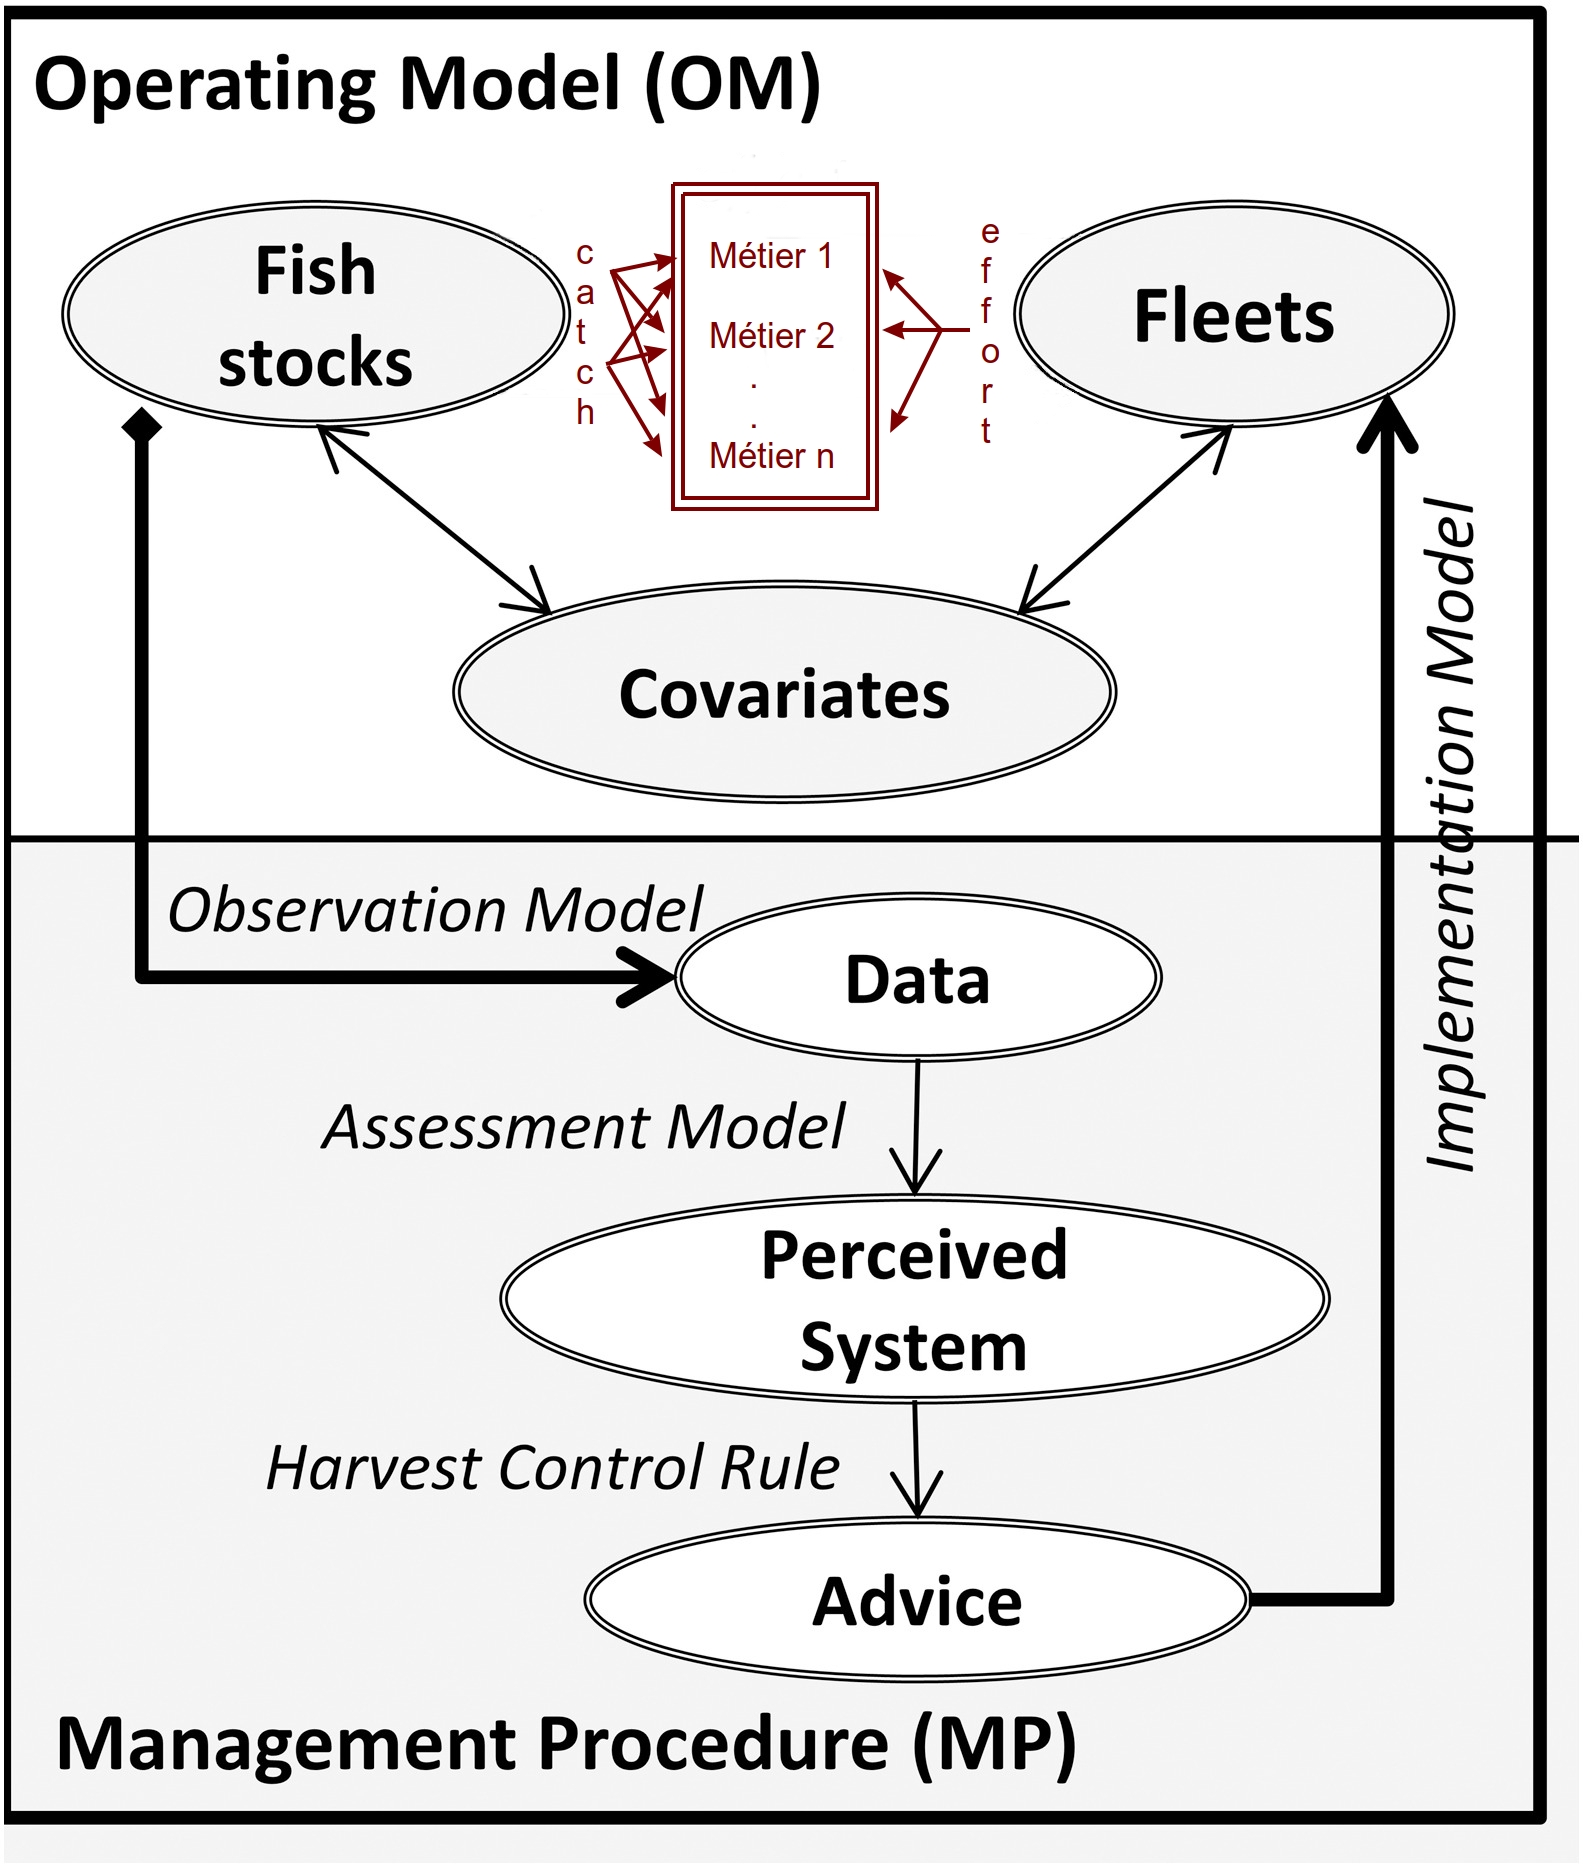
\includegraphics[width=0.6\linewidth]{figures/FLBEIA}
	\caption{FLBEIA schematic, adapted from \cite{Garcia2017} to show the
		métier interaction (dark red) in the modelling framework.} 
	\label{fig:flbeia}
\end{figure}	


\begin{figure}[!ht]
	\centering
\begin{subfigure}
	\centering
	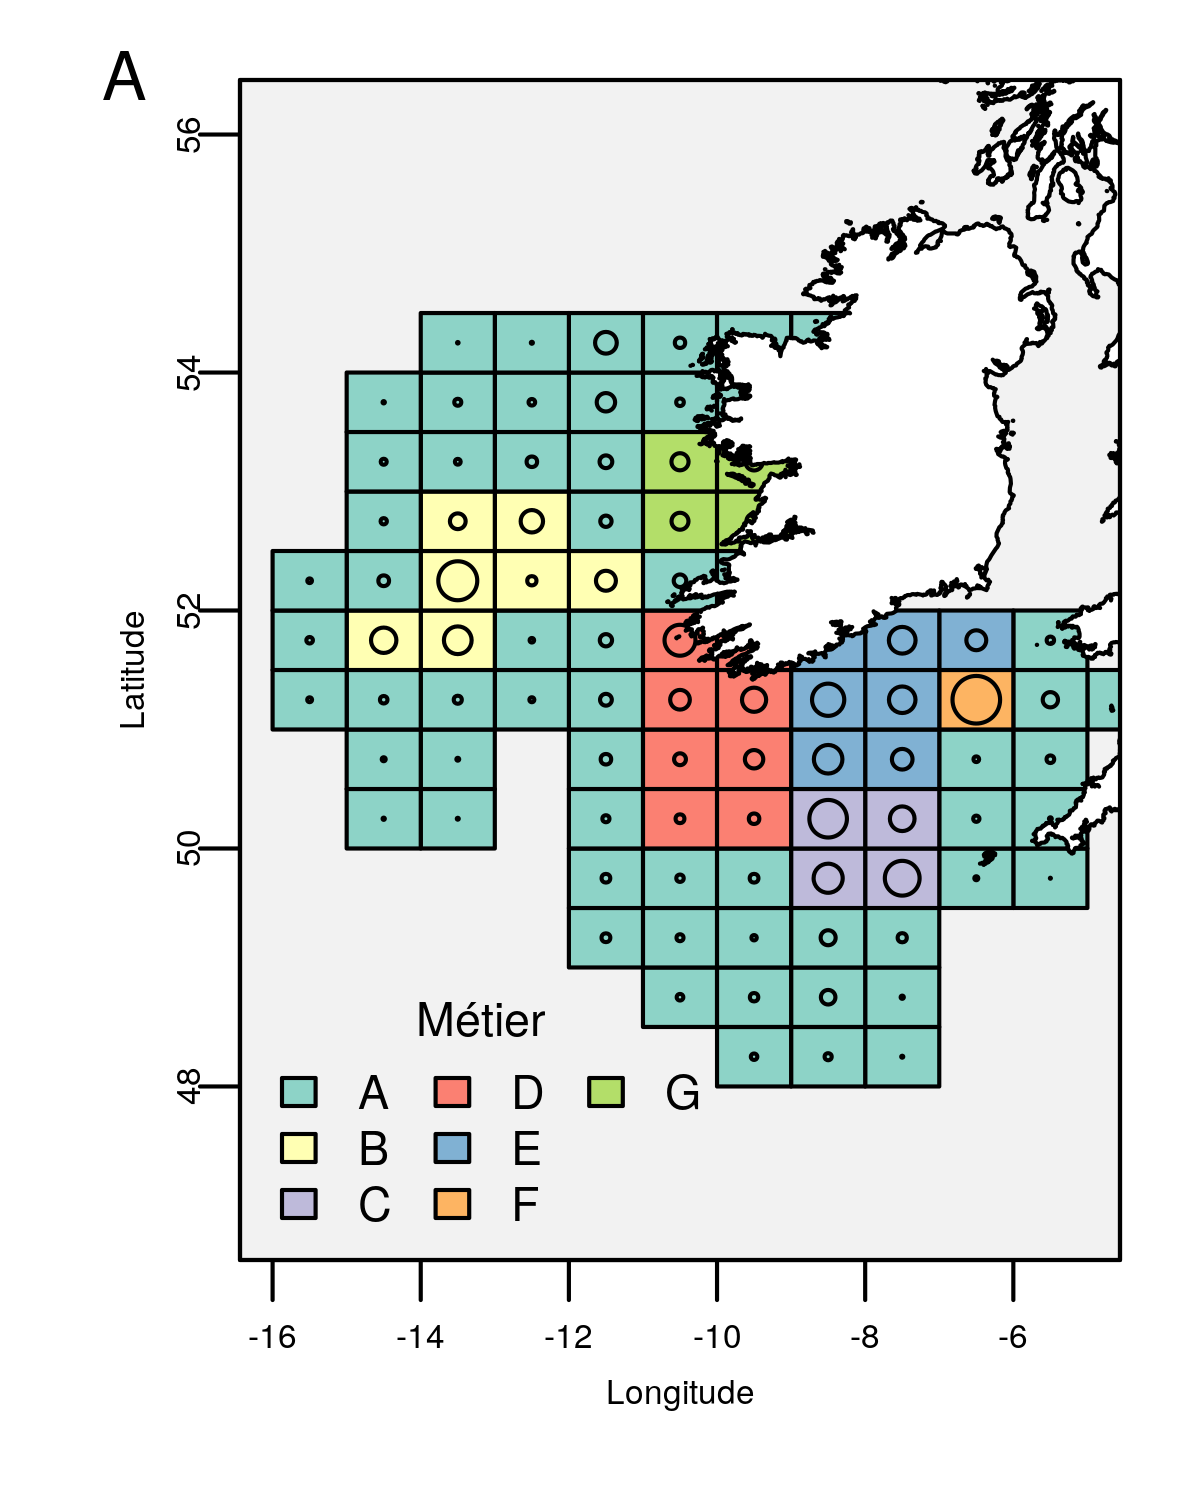
\includegraphics[width=0.6\linewidth]{figures/Final_Metier_locations}
\end{subfigure}
\begin{subfigure}
	\centering
	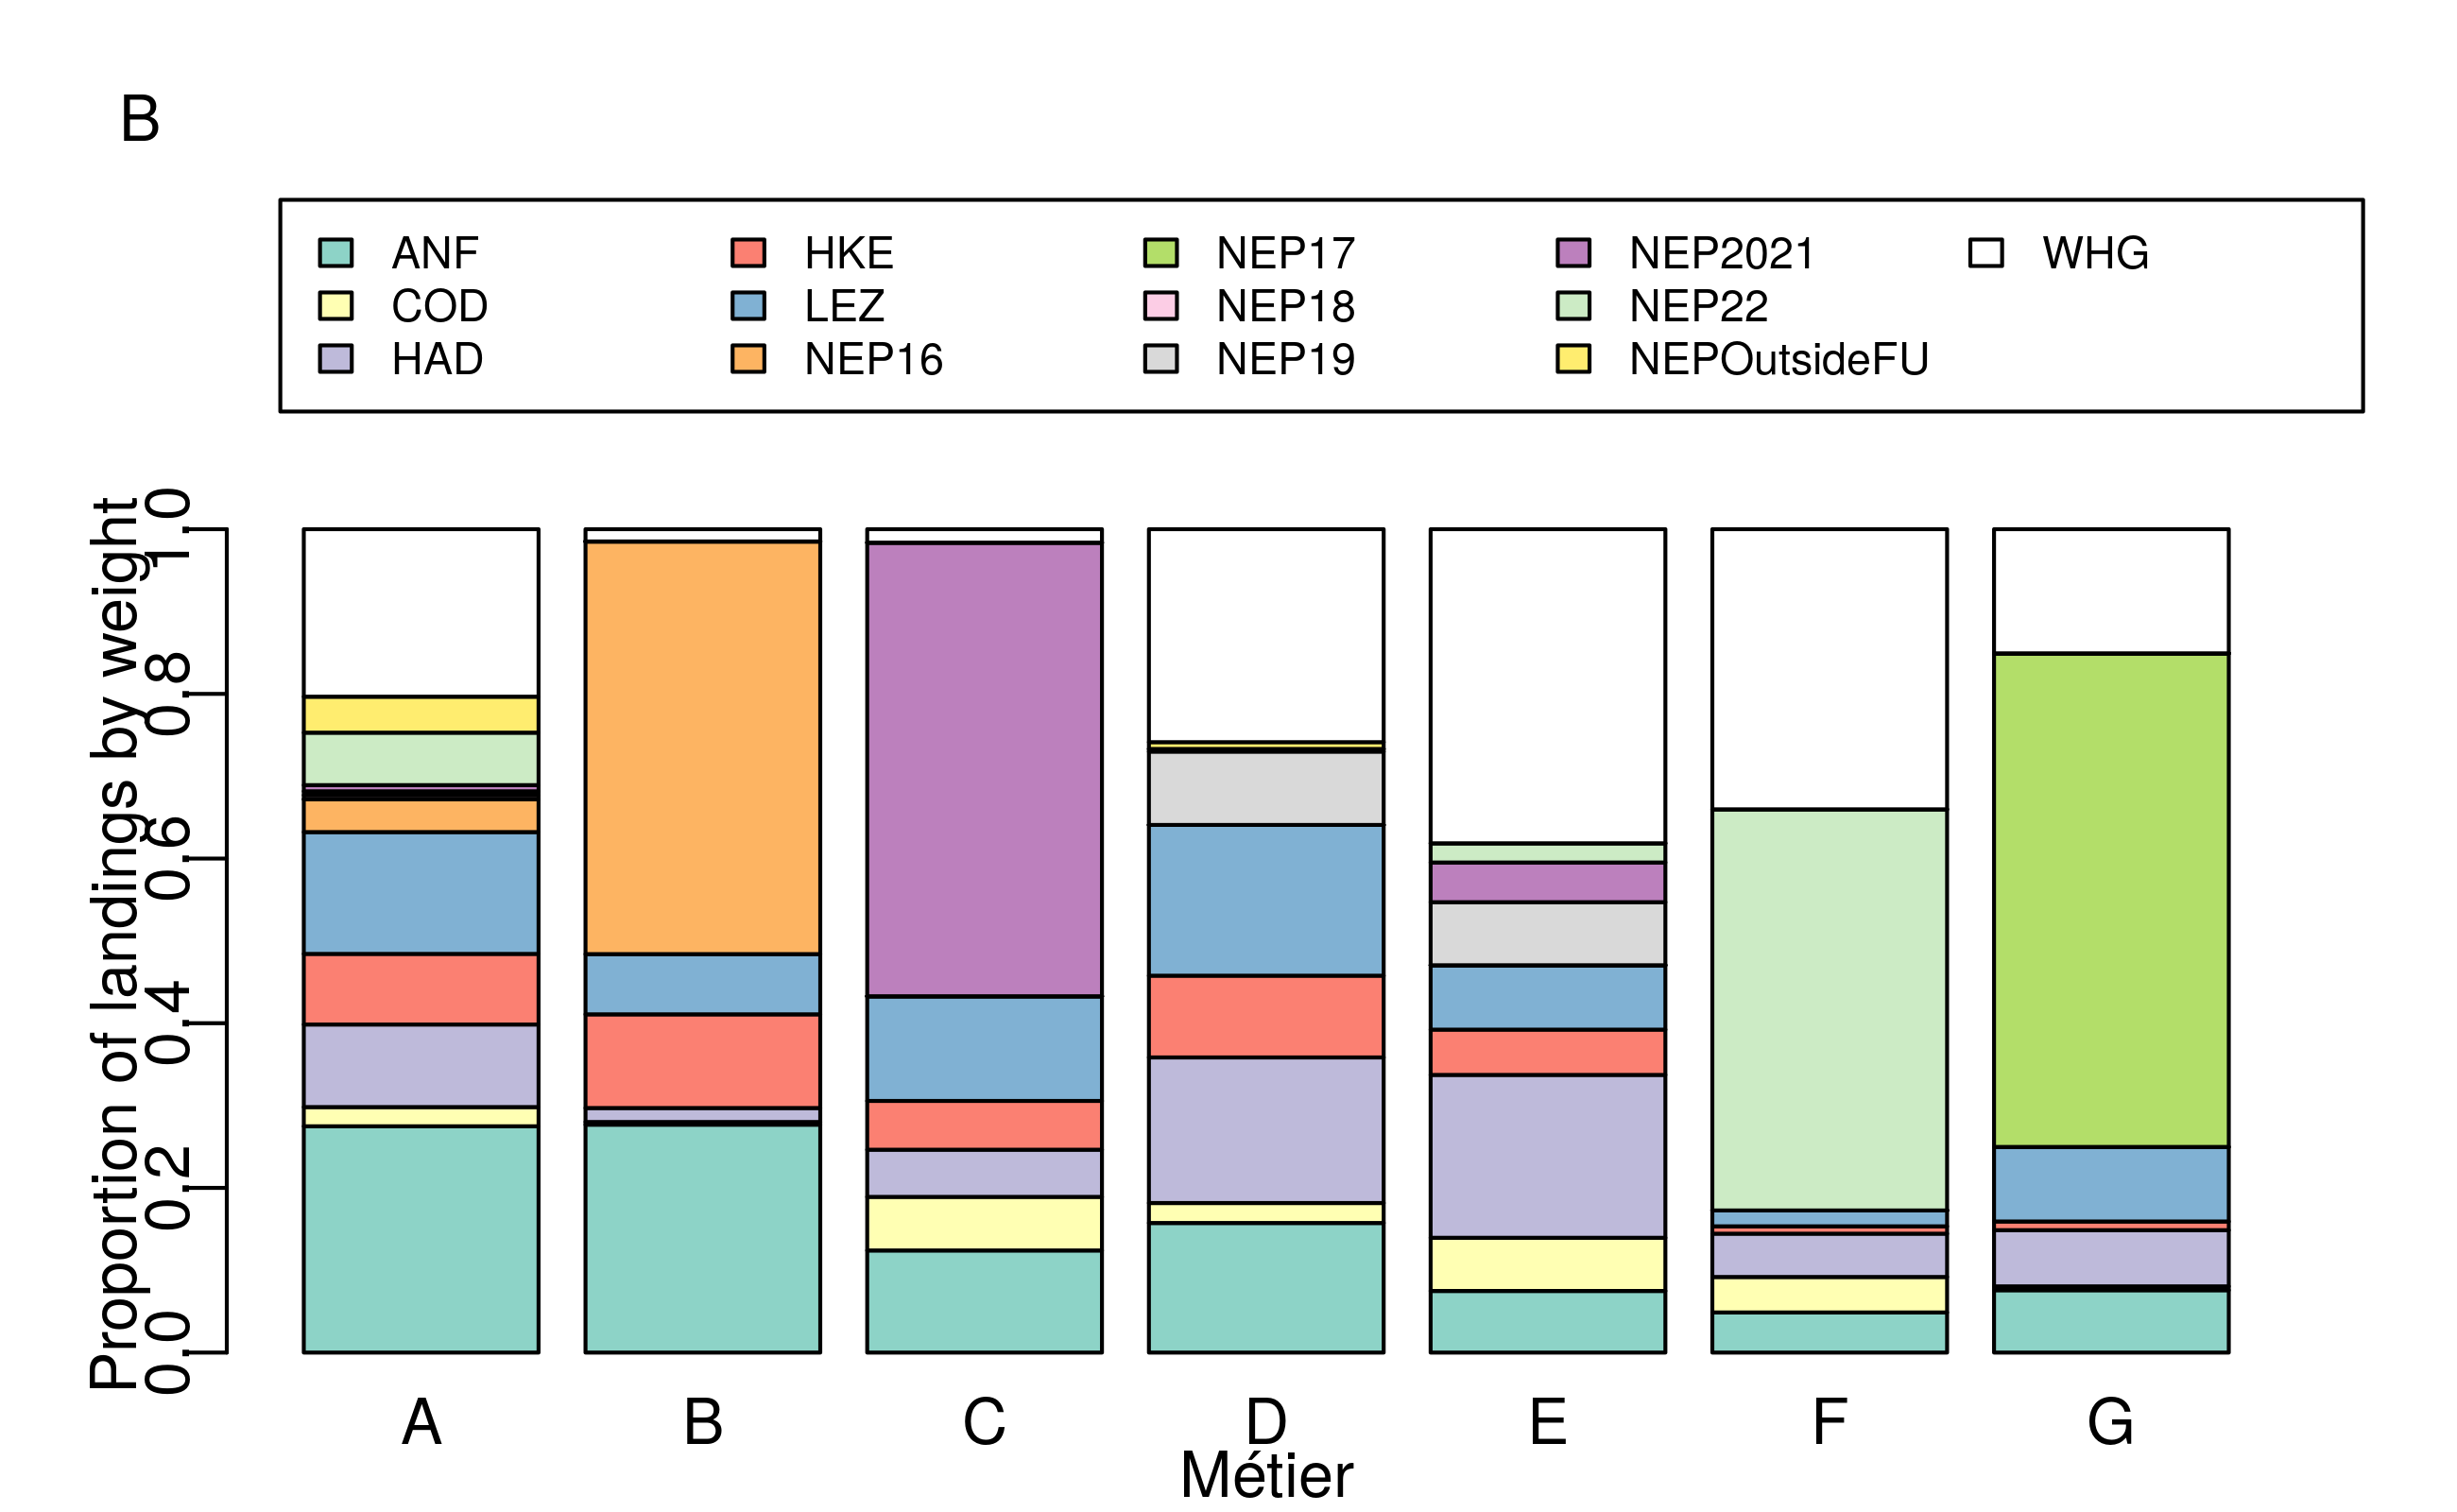
\includegraphics[width=0.8\linewidth]{figures/Final_Metier_catchcomp}
\end{subfigure}
\caption{The métier defined through spatial clustering of similar catch
	composition for Irish Otter trawlers modified by using knowledge of
	fishing grounds to make coherent spatial units. The circles represent
	relative fishing effort in each of the rectangles. Catch compositions
	for the métier indicating the dominant stocks in catches for each of
	the fishing grounds. Stock codes in Table \ref{tab:brp}.} 
	\label{fig:metier}

\end{figure}	

\newpage

\begin{sidewaysfigure}[!ht]
	\centering
	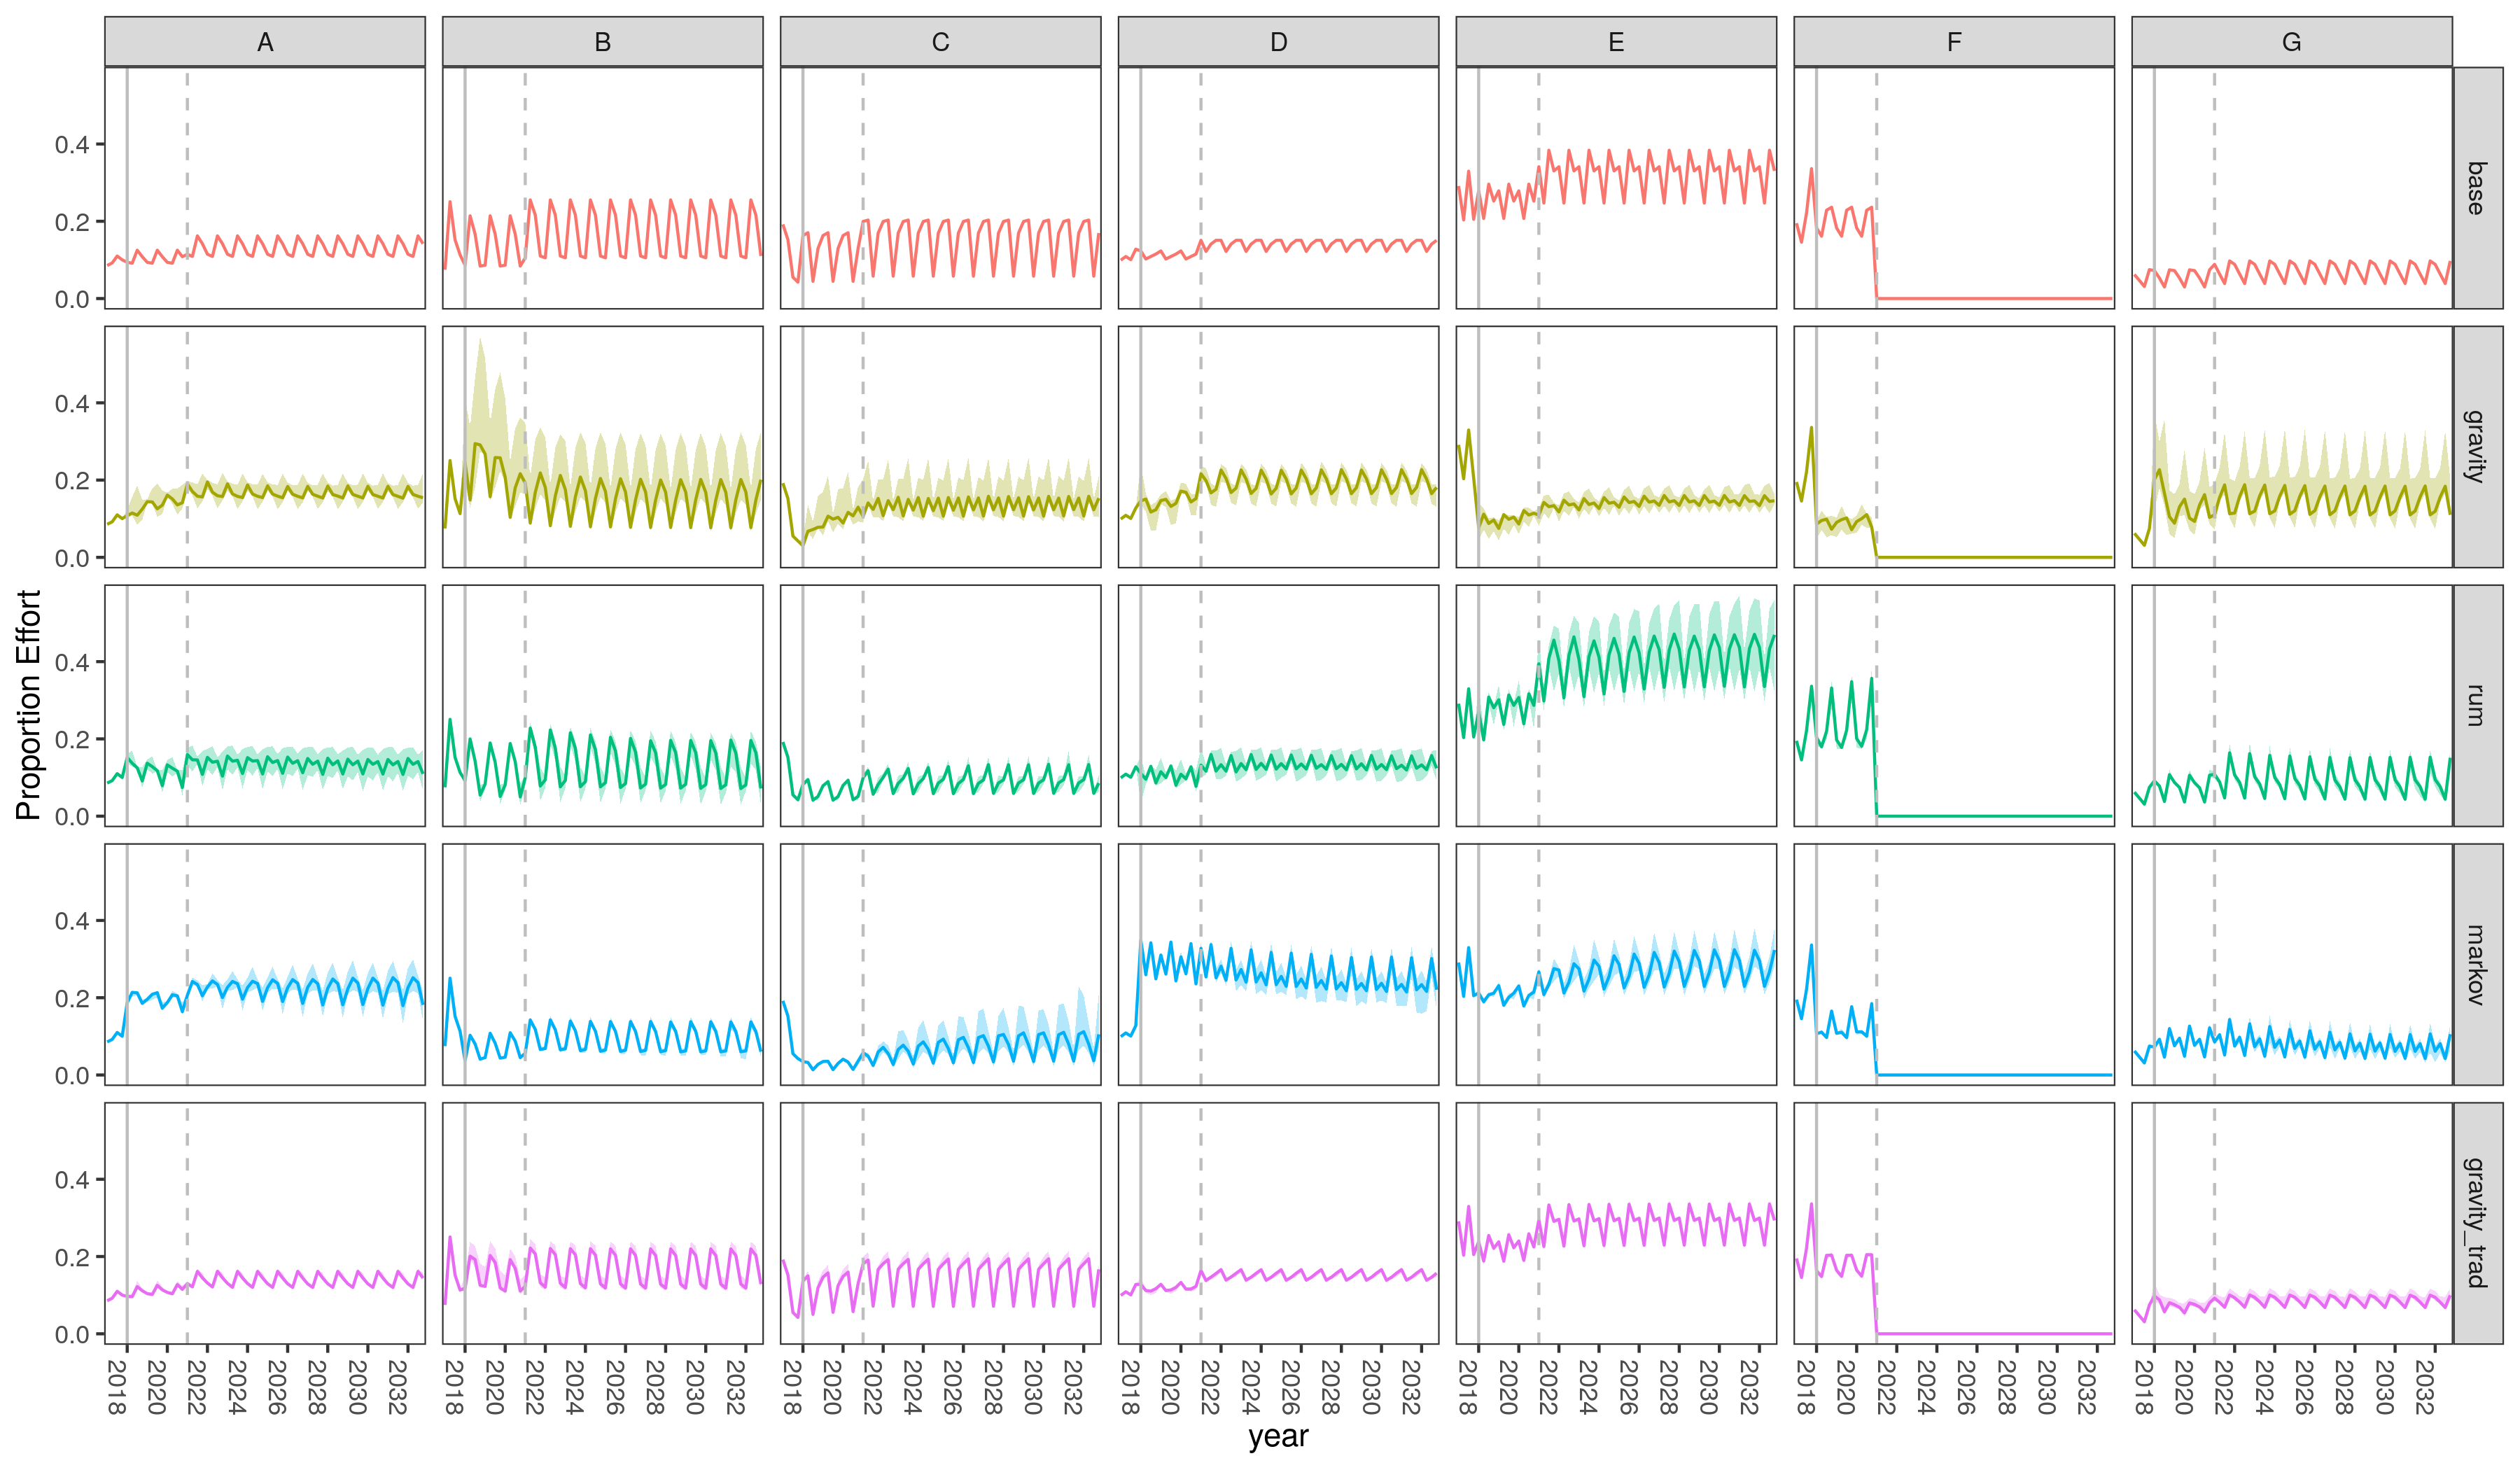
\includegraphics[width=1\linewidth]{figures/Effort_shares}
	\caption{Quarterly fishing effort share (proportion) for each métier
		and location choice model (2017 - 2032). Light shading
		represents 5\% and 95\% variability due to recruitment and
		catchability. Solid line indicates end of the data/start of
		simulations and the dashed line the implementation of the
		spatial closure.} 
	\label{fig:effort}
\end{sidewaysfigure}	

\newpage

\begin{figure}[!ht]
	\centering
	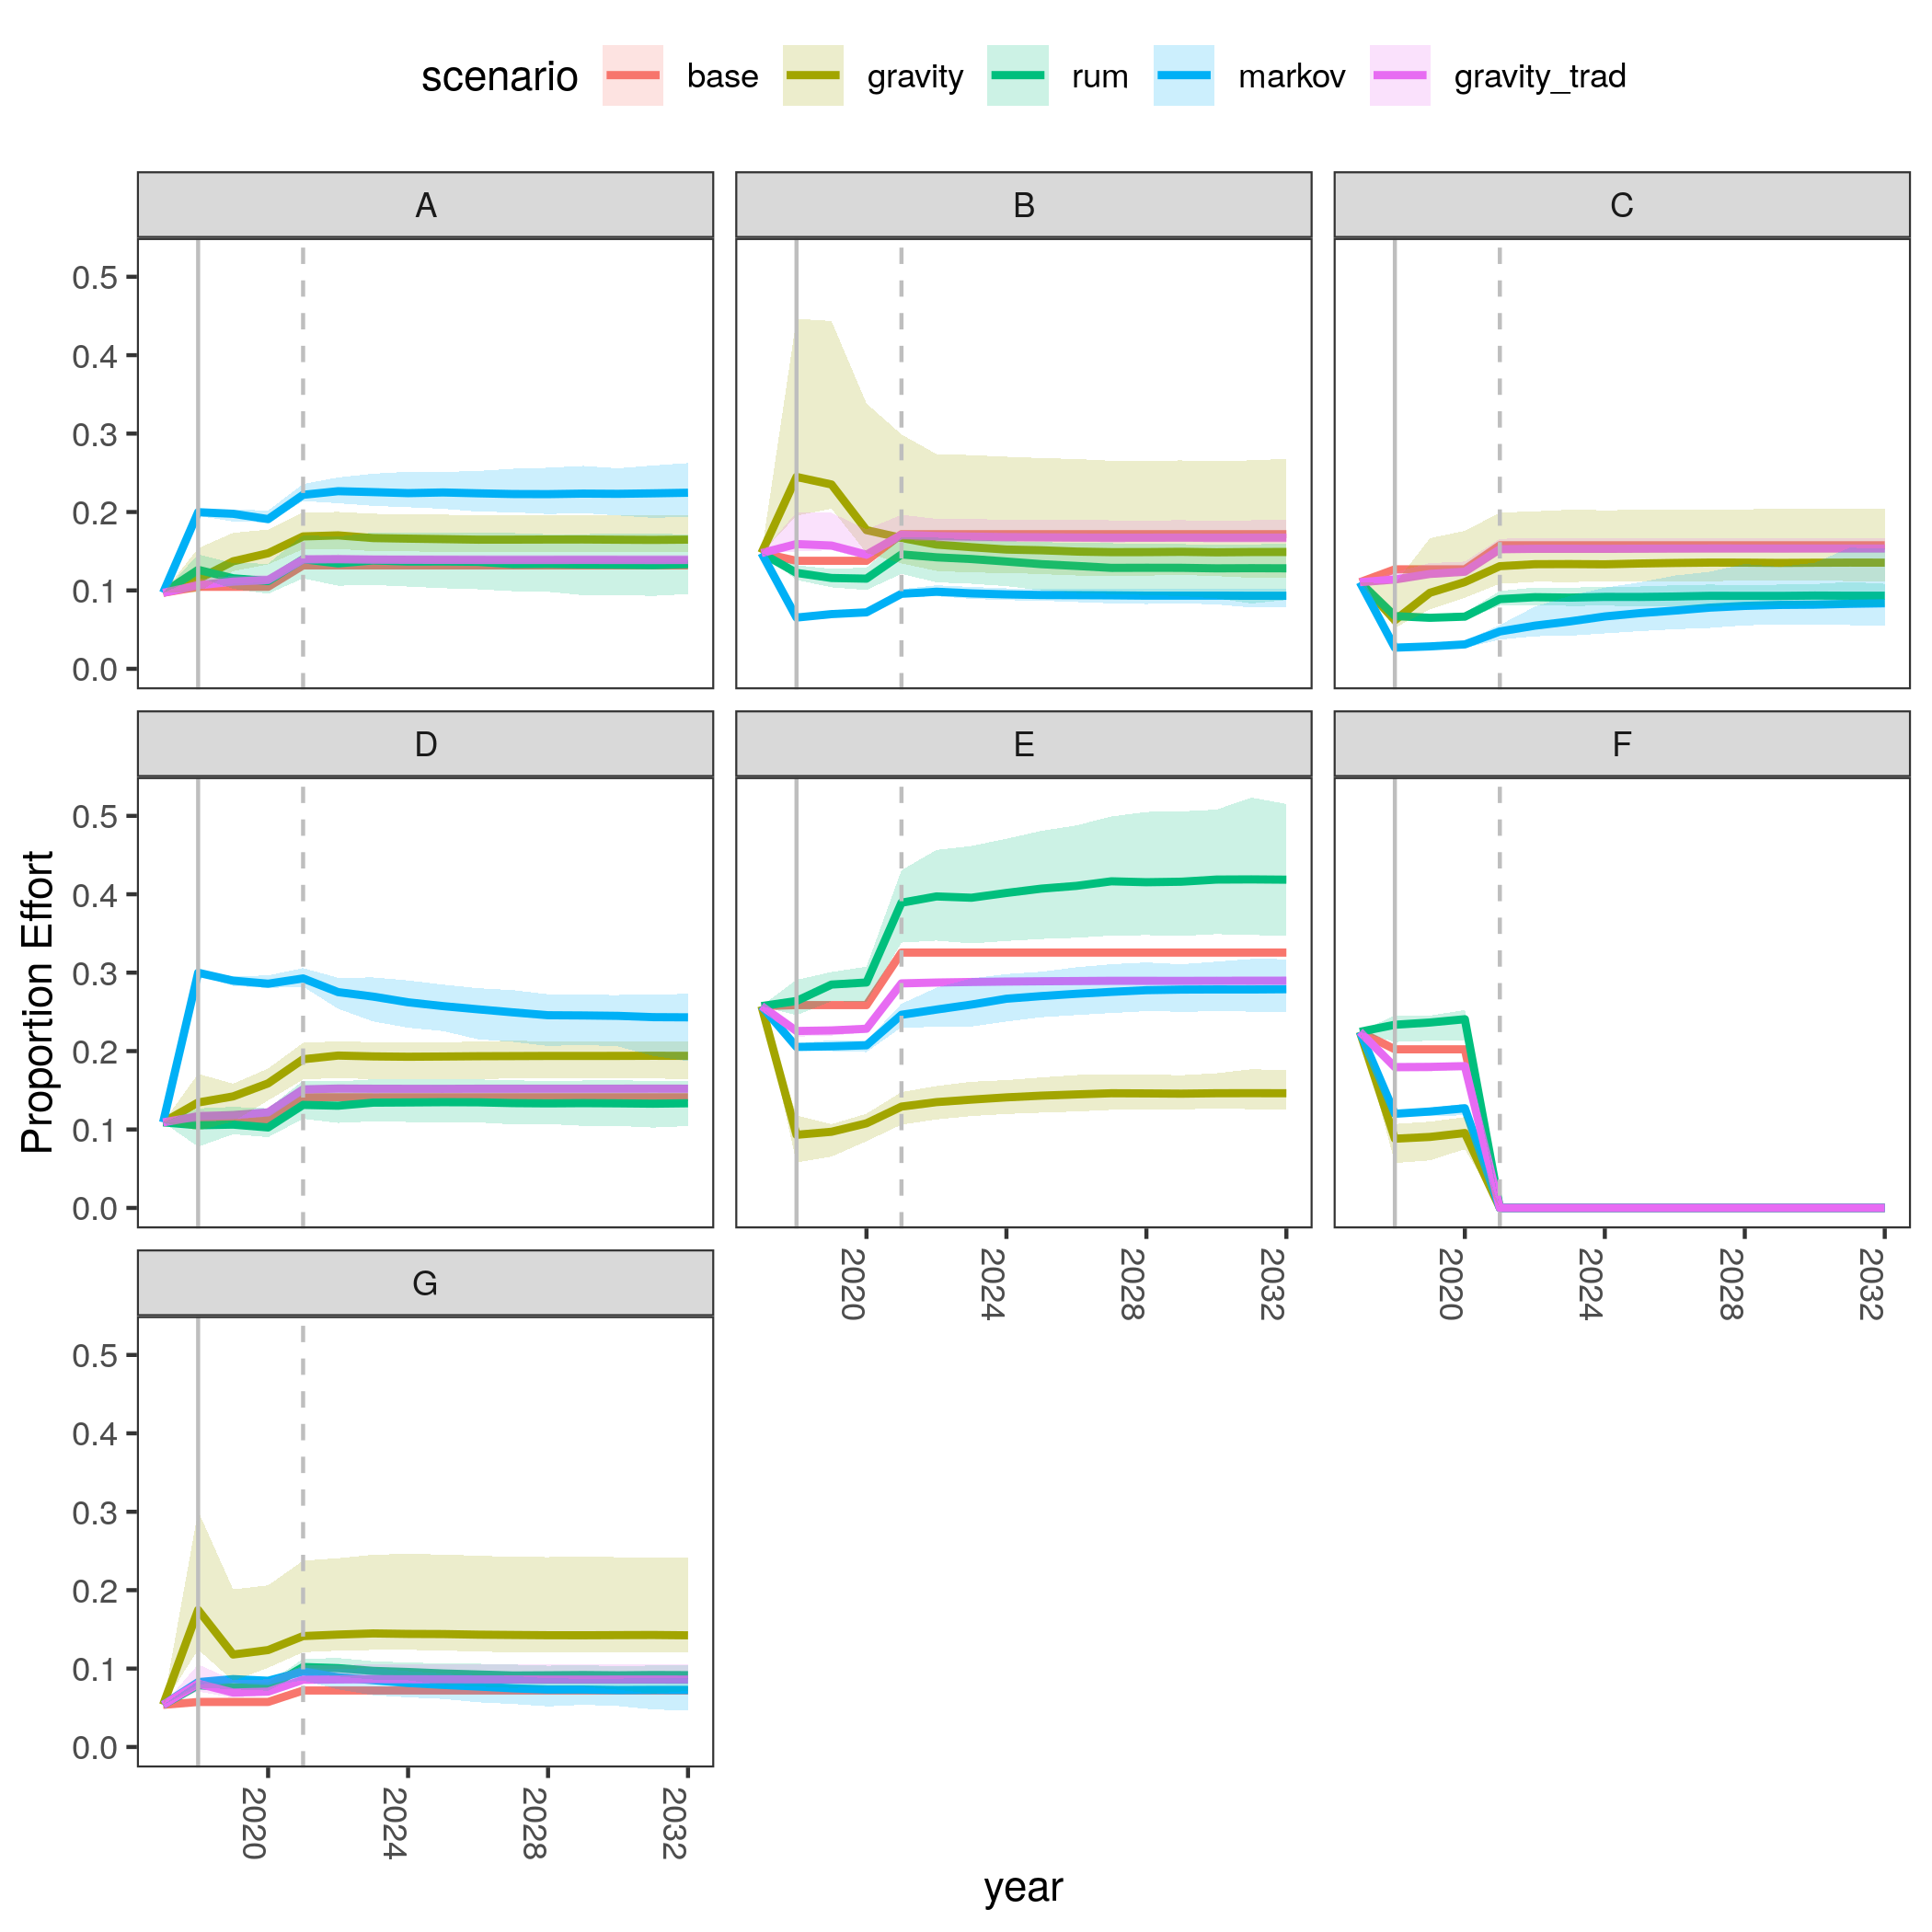
\includegraphics[width=1\linewidth]{figures/Effort_shares_annual}
	\caption{Annualised effort share (proportion) for each métier
		and location choice model (2017 - 2032). Light shading
		represents 5\% and 95\% variability due to recruitment and
		catchability. Solid line indicates end of the data/start of
		simulations and the dashed line the implementation of the
		spatial closure.} 
	\label{fig:effort_an}
\end{figure}	

\begin{figure}[!ht]
	\centering
	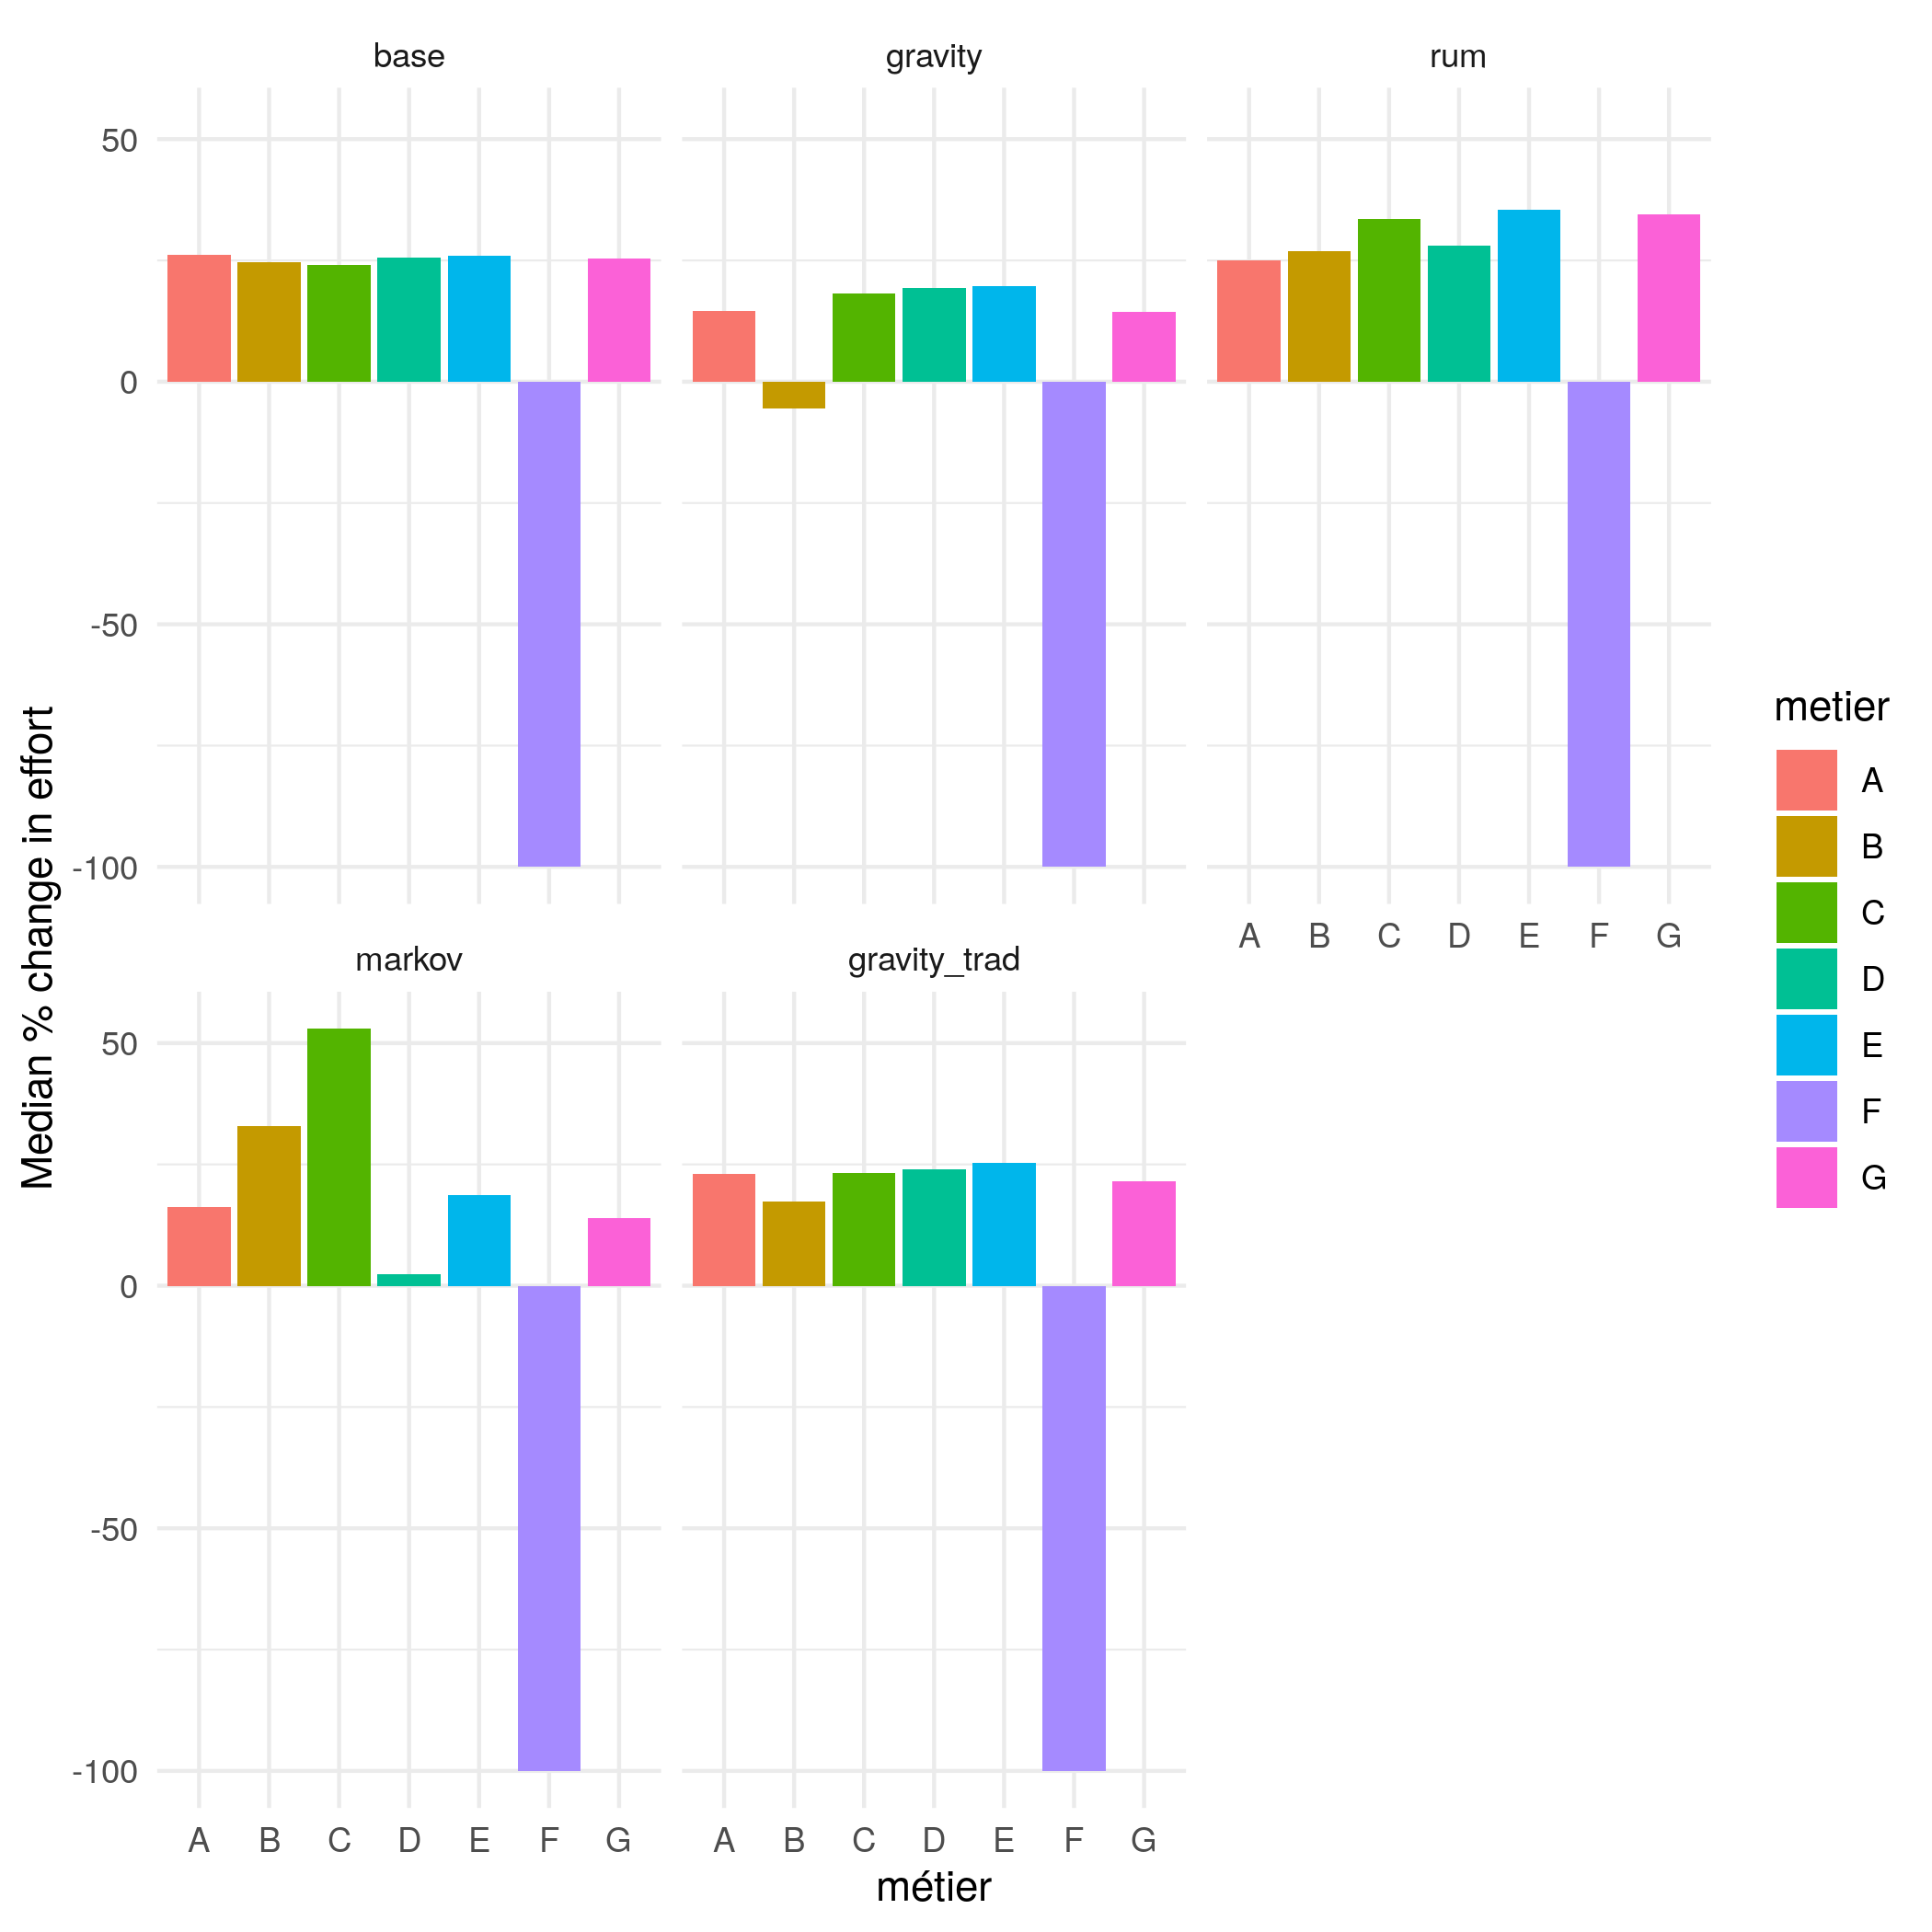
\includegraphics[width=1\linewidth]{figures/Change_effort}
	\caption{Percentage change in annualised effort share for each of the
		métier from before (2020) the closure of métier F and first
		year of the closure (2021).} 
	\label{fig:effort_chg}
\end{figure}	

\begin{figure}[!ht]
	\centering
	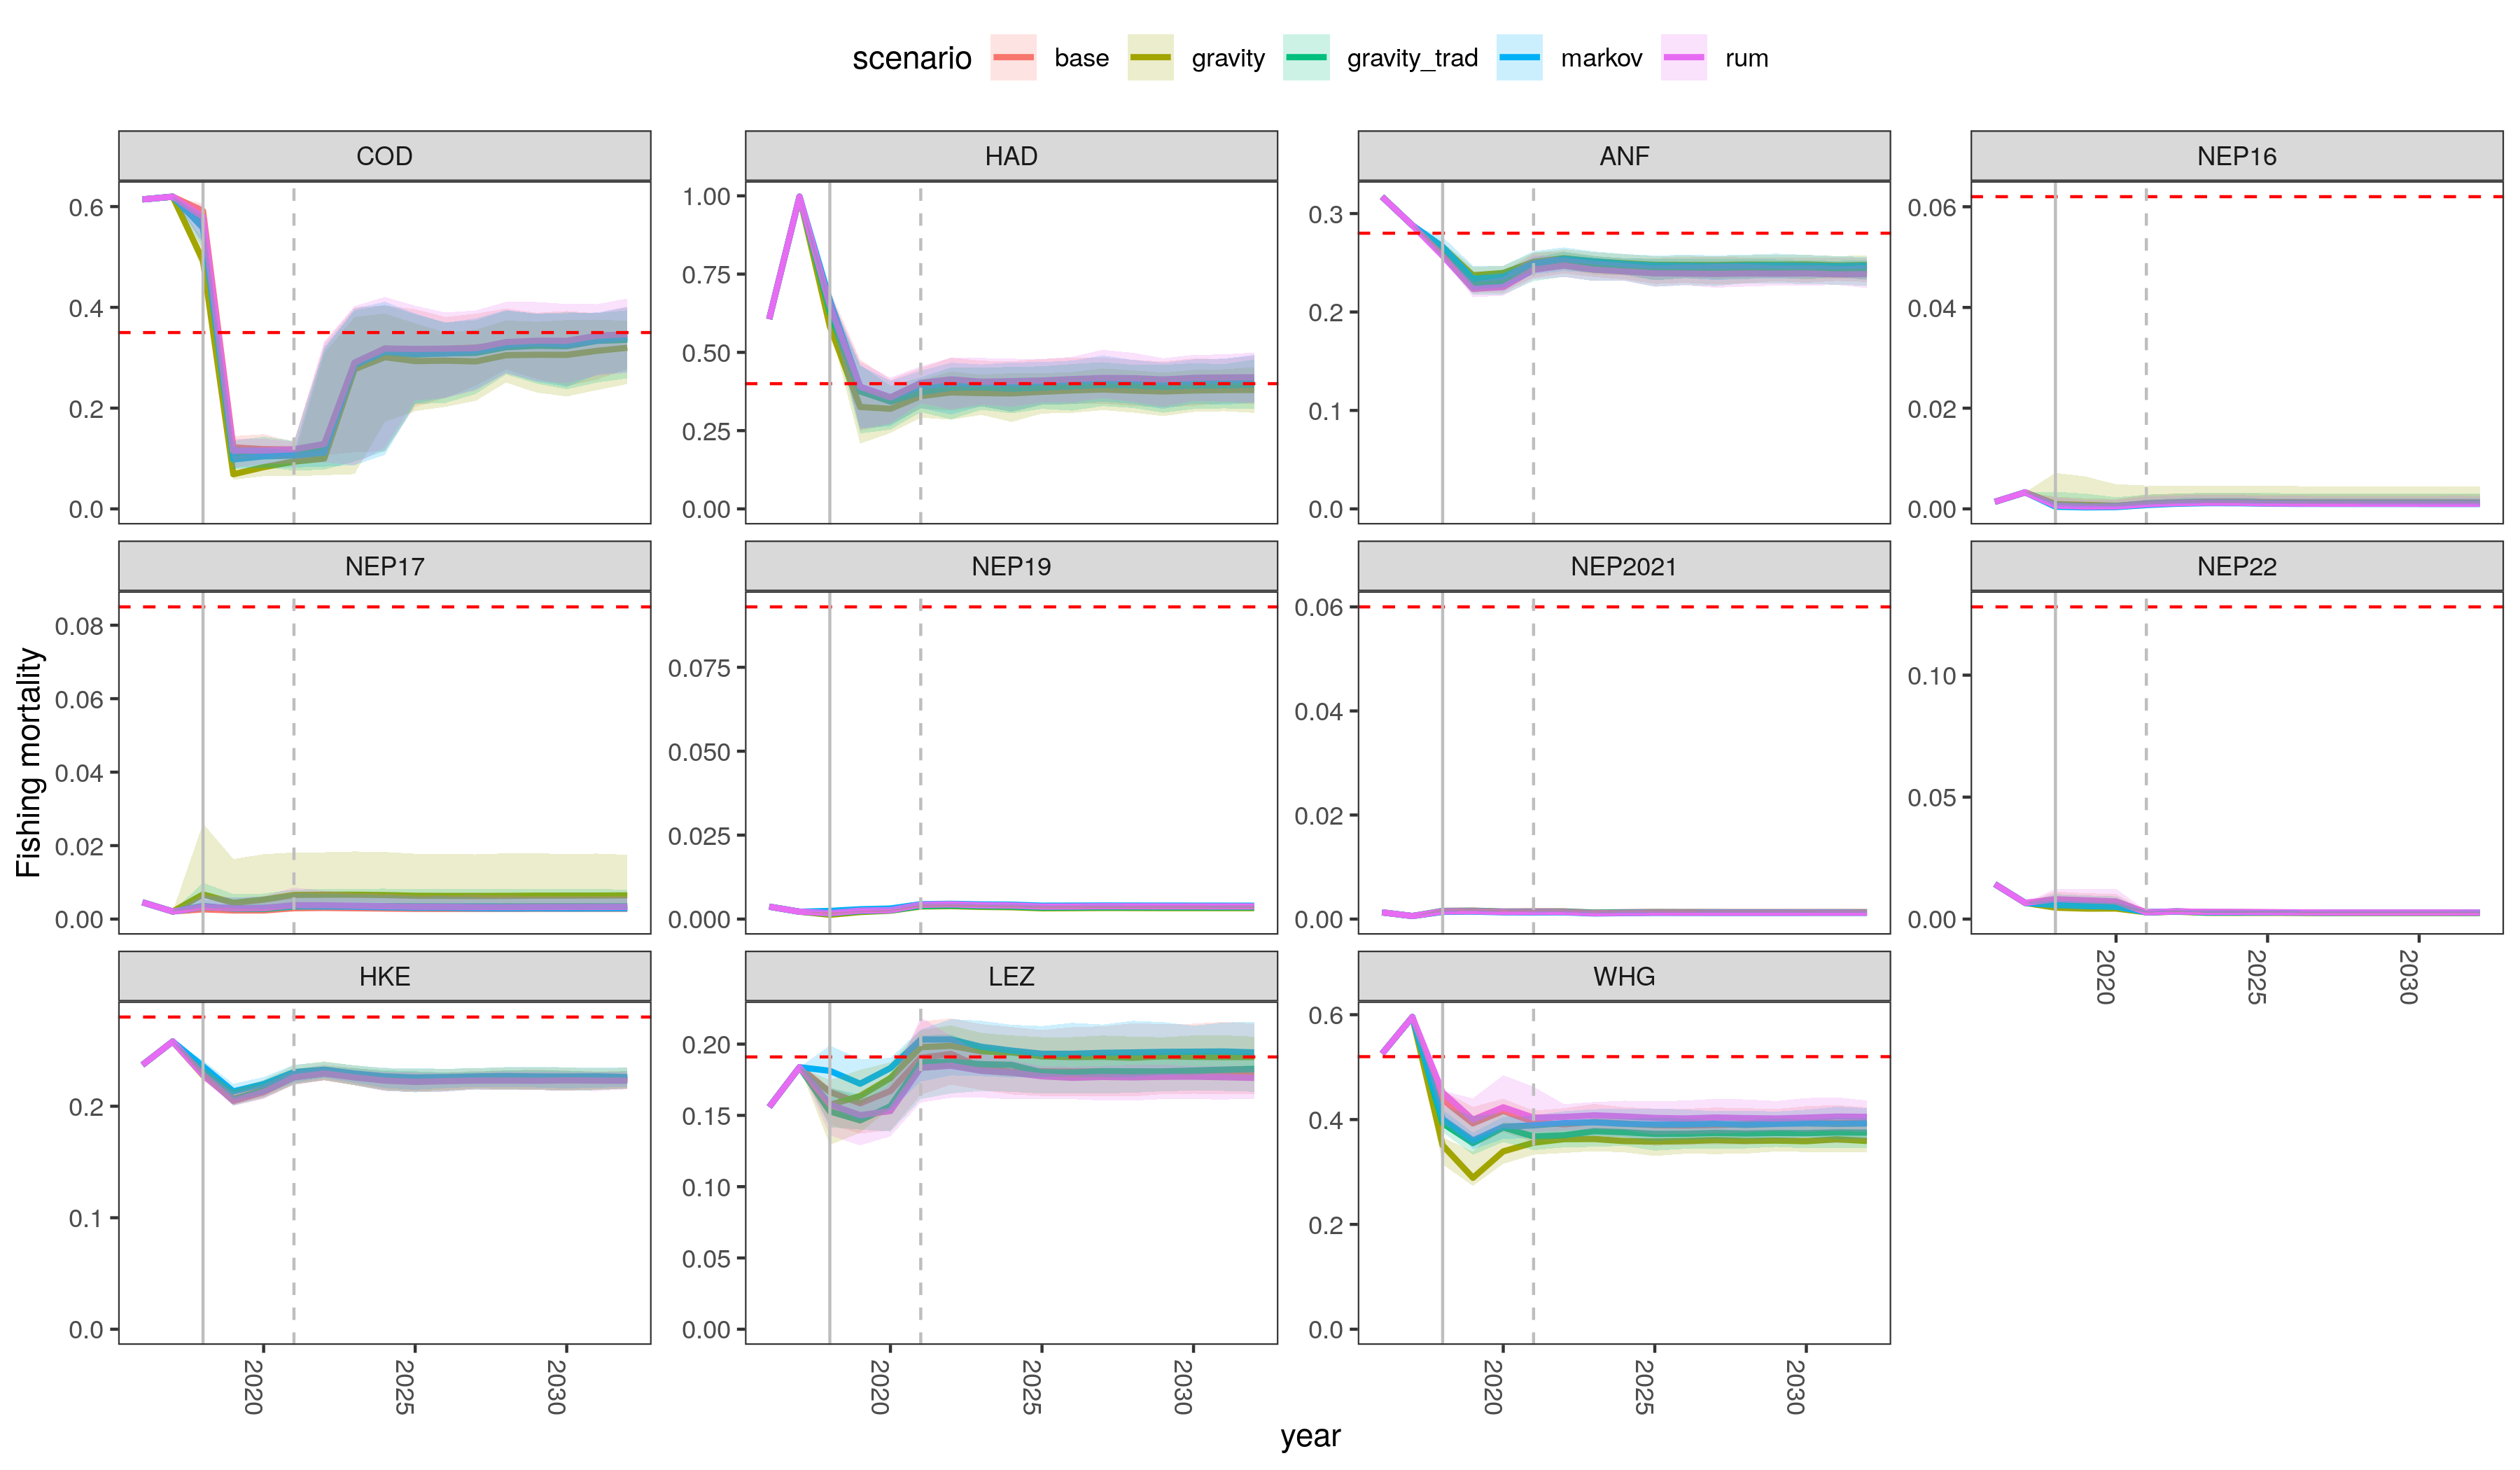
\includegraphics[width=1\linewidth]{figures/F_difference}
	\caption{Fishing mortality for each stock under the different location
		choice models. Each stock was targeted to be fished at its Fmsy
		rate, using the ICES MSY Harvest Control Rule. Light shading
		represents 5\% and 95\% variability due to recruitment and
		catchability. Solid line indicates end of the data/start of
		simulations and the dashed line the implementation of the
		spatial closure. Dashed red lines indicate the stock Fmsy
		reference point.} 
	\label{fig:F}
\end{figure}	

\begin{figure}[!ht]
	\centering
	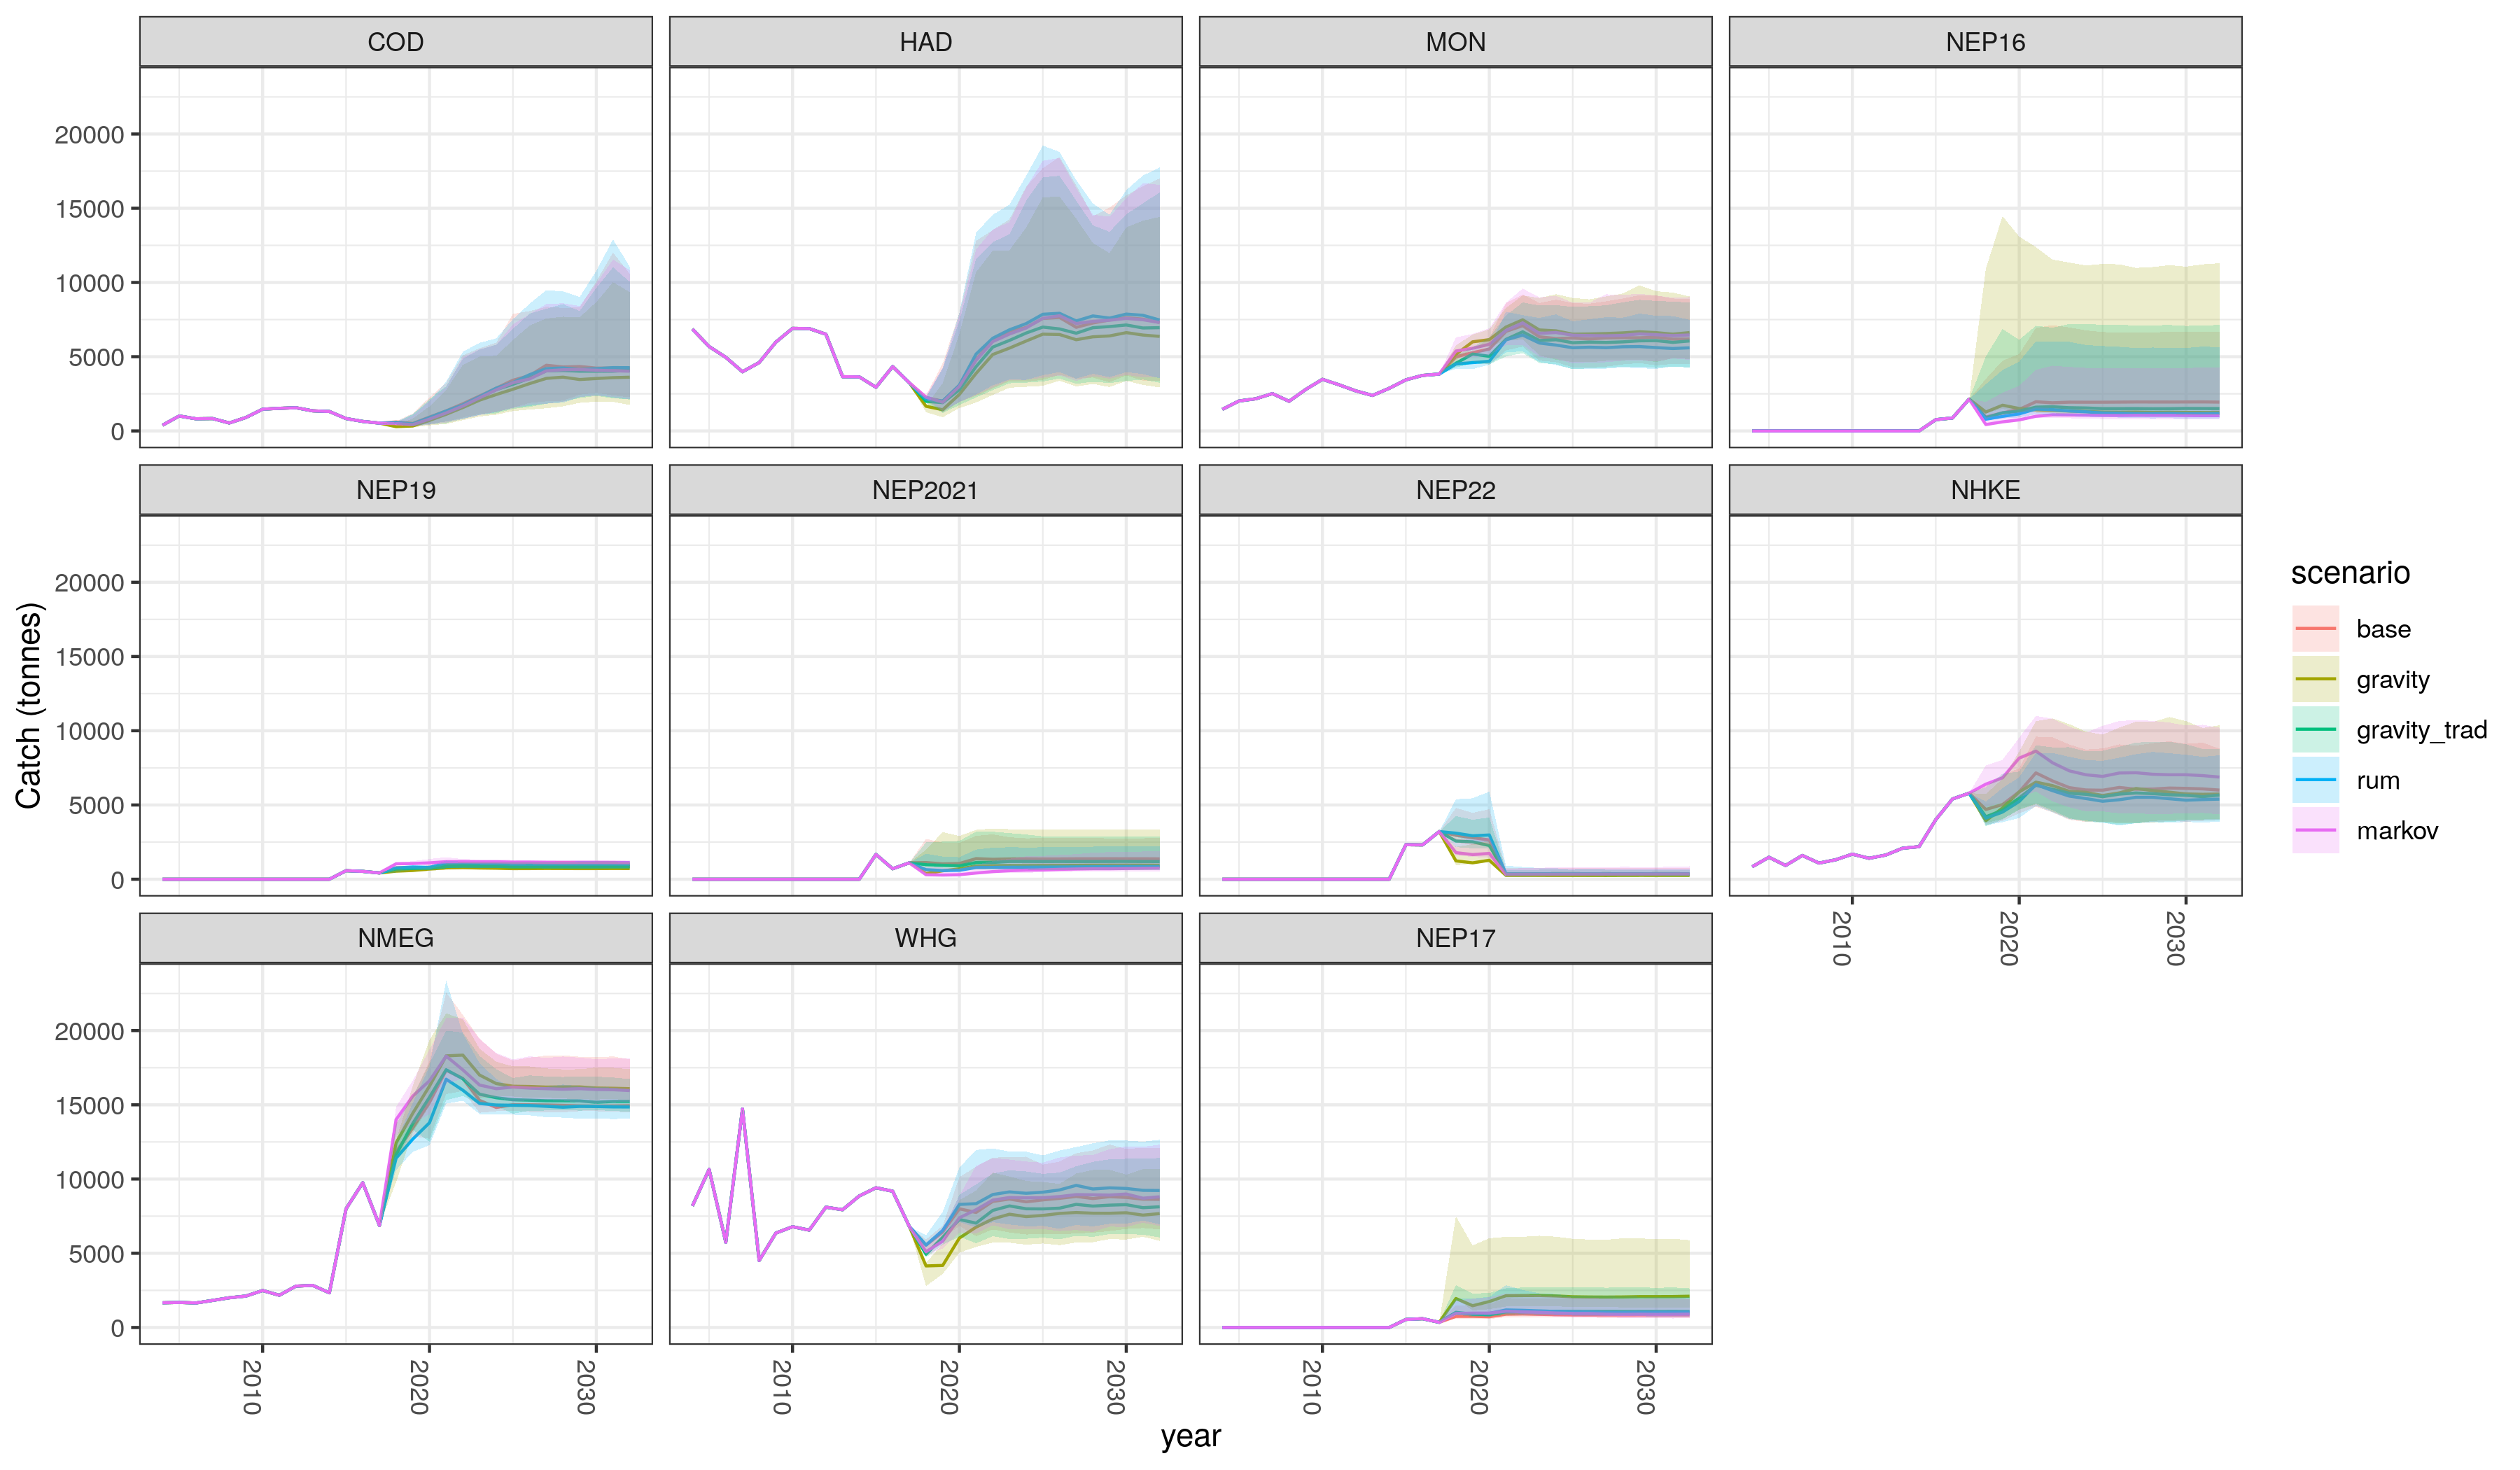
\includegraphics[width=1\linewidth]{figures/IE_Otter_catches}
	\caption{Catches of each stock by Irish Otter trawlers under the
		different location choice models. Light shading represents 5\%
		and 95\% variability due to recruitment and catchability. Solid
		line indicates end of the data/start of simulations and the
		dashed line the implementation of the spatial closure.} 
	\label{fig:OtterC}
\end{figure}	

\begin{figure}[!ht]
	\centering
	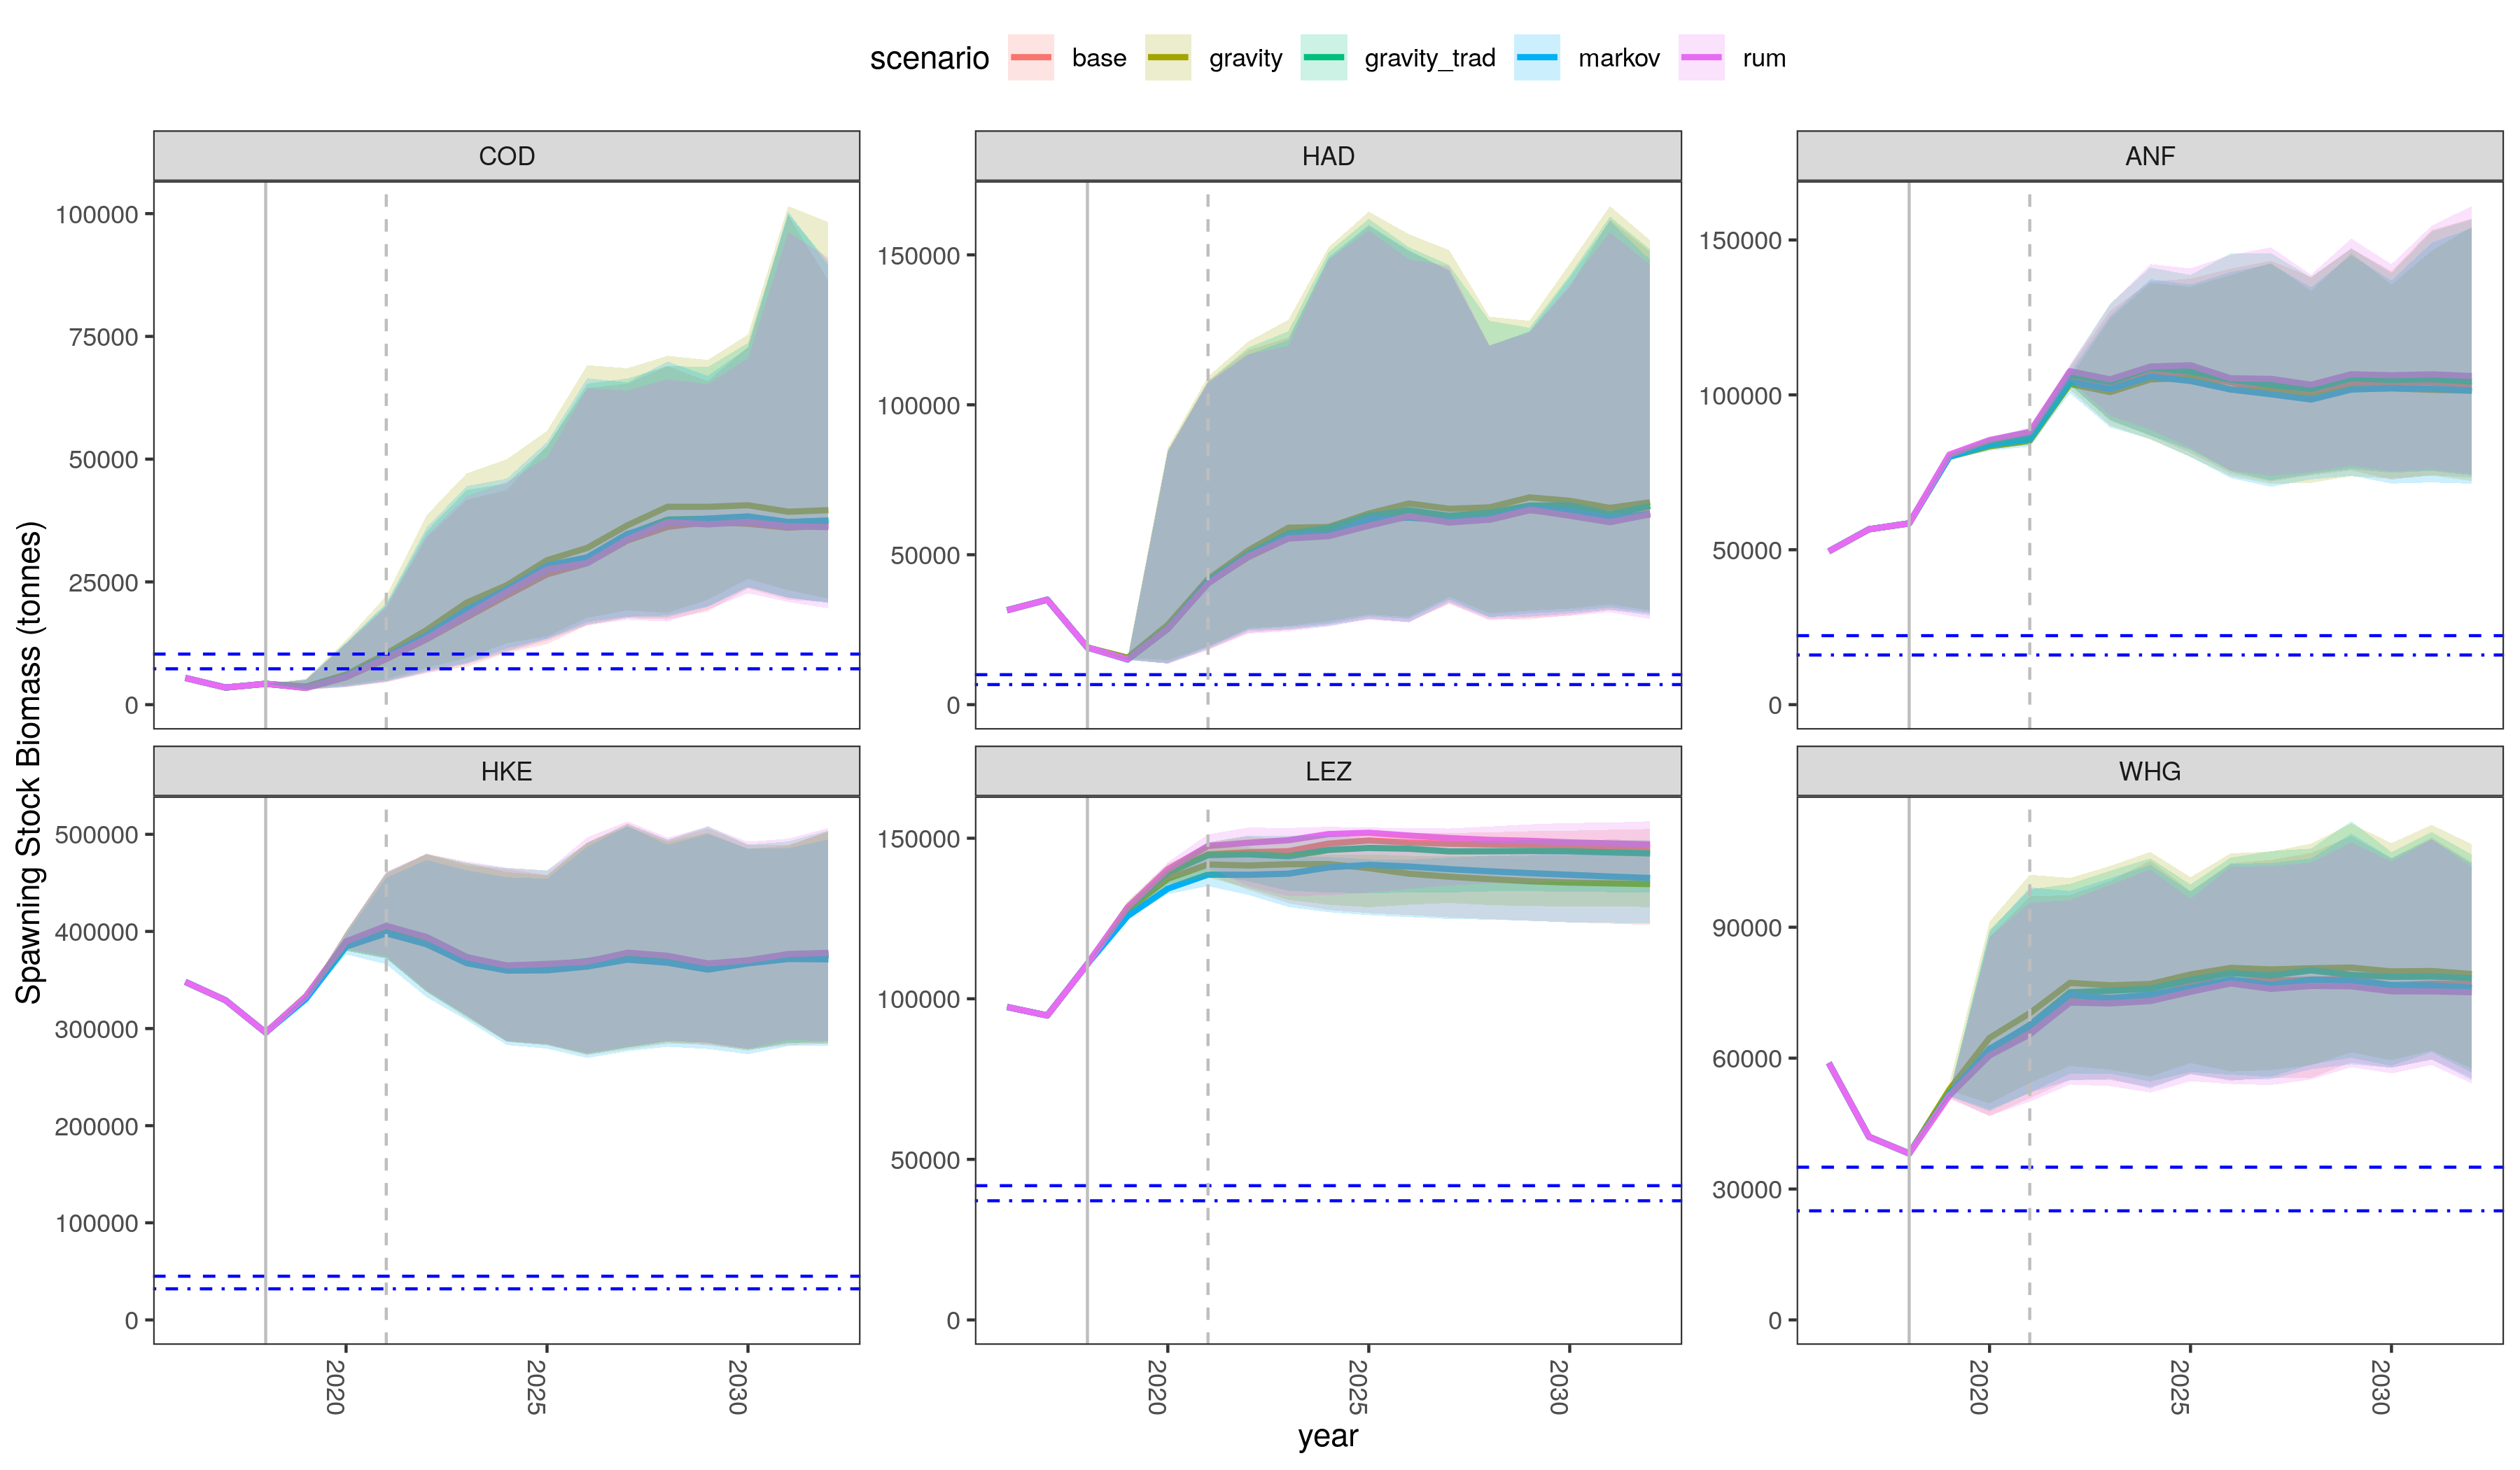
\includegraphics[width=1\linewidth]{figures/SSB_difference}
	\caption{Spawning Stock Biomass for the fish stocks under each location
		model scenario. Light shading represents 5\% and 95\%
		variability due to recruitment and catchability. Solid line
		indicates end of the data/start of simulations and the dashed
		line the implementation of the spatial closure.  Dotdashed and
		dashed blue lines indicate the Blim reference and Bmsytrigger
		reference points respectively.} 
	\label{fig:SSB}
\end{figure}	

\begin{figure}[!ht]
	\centering
	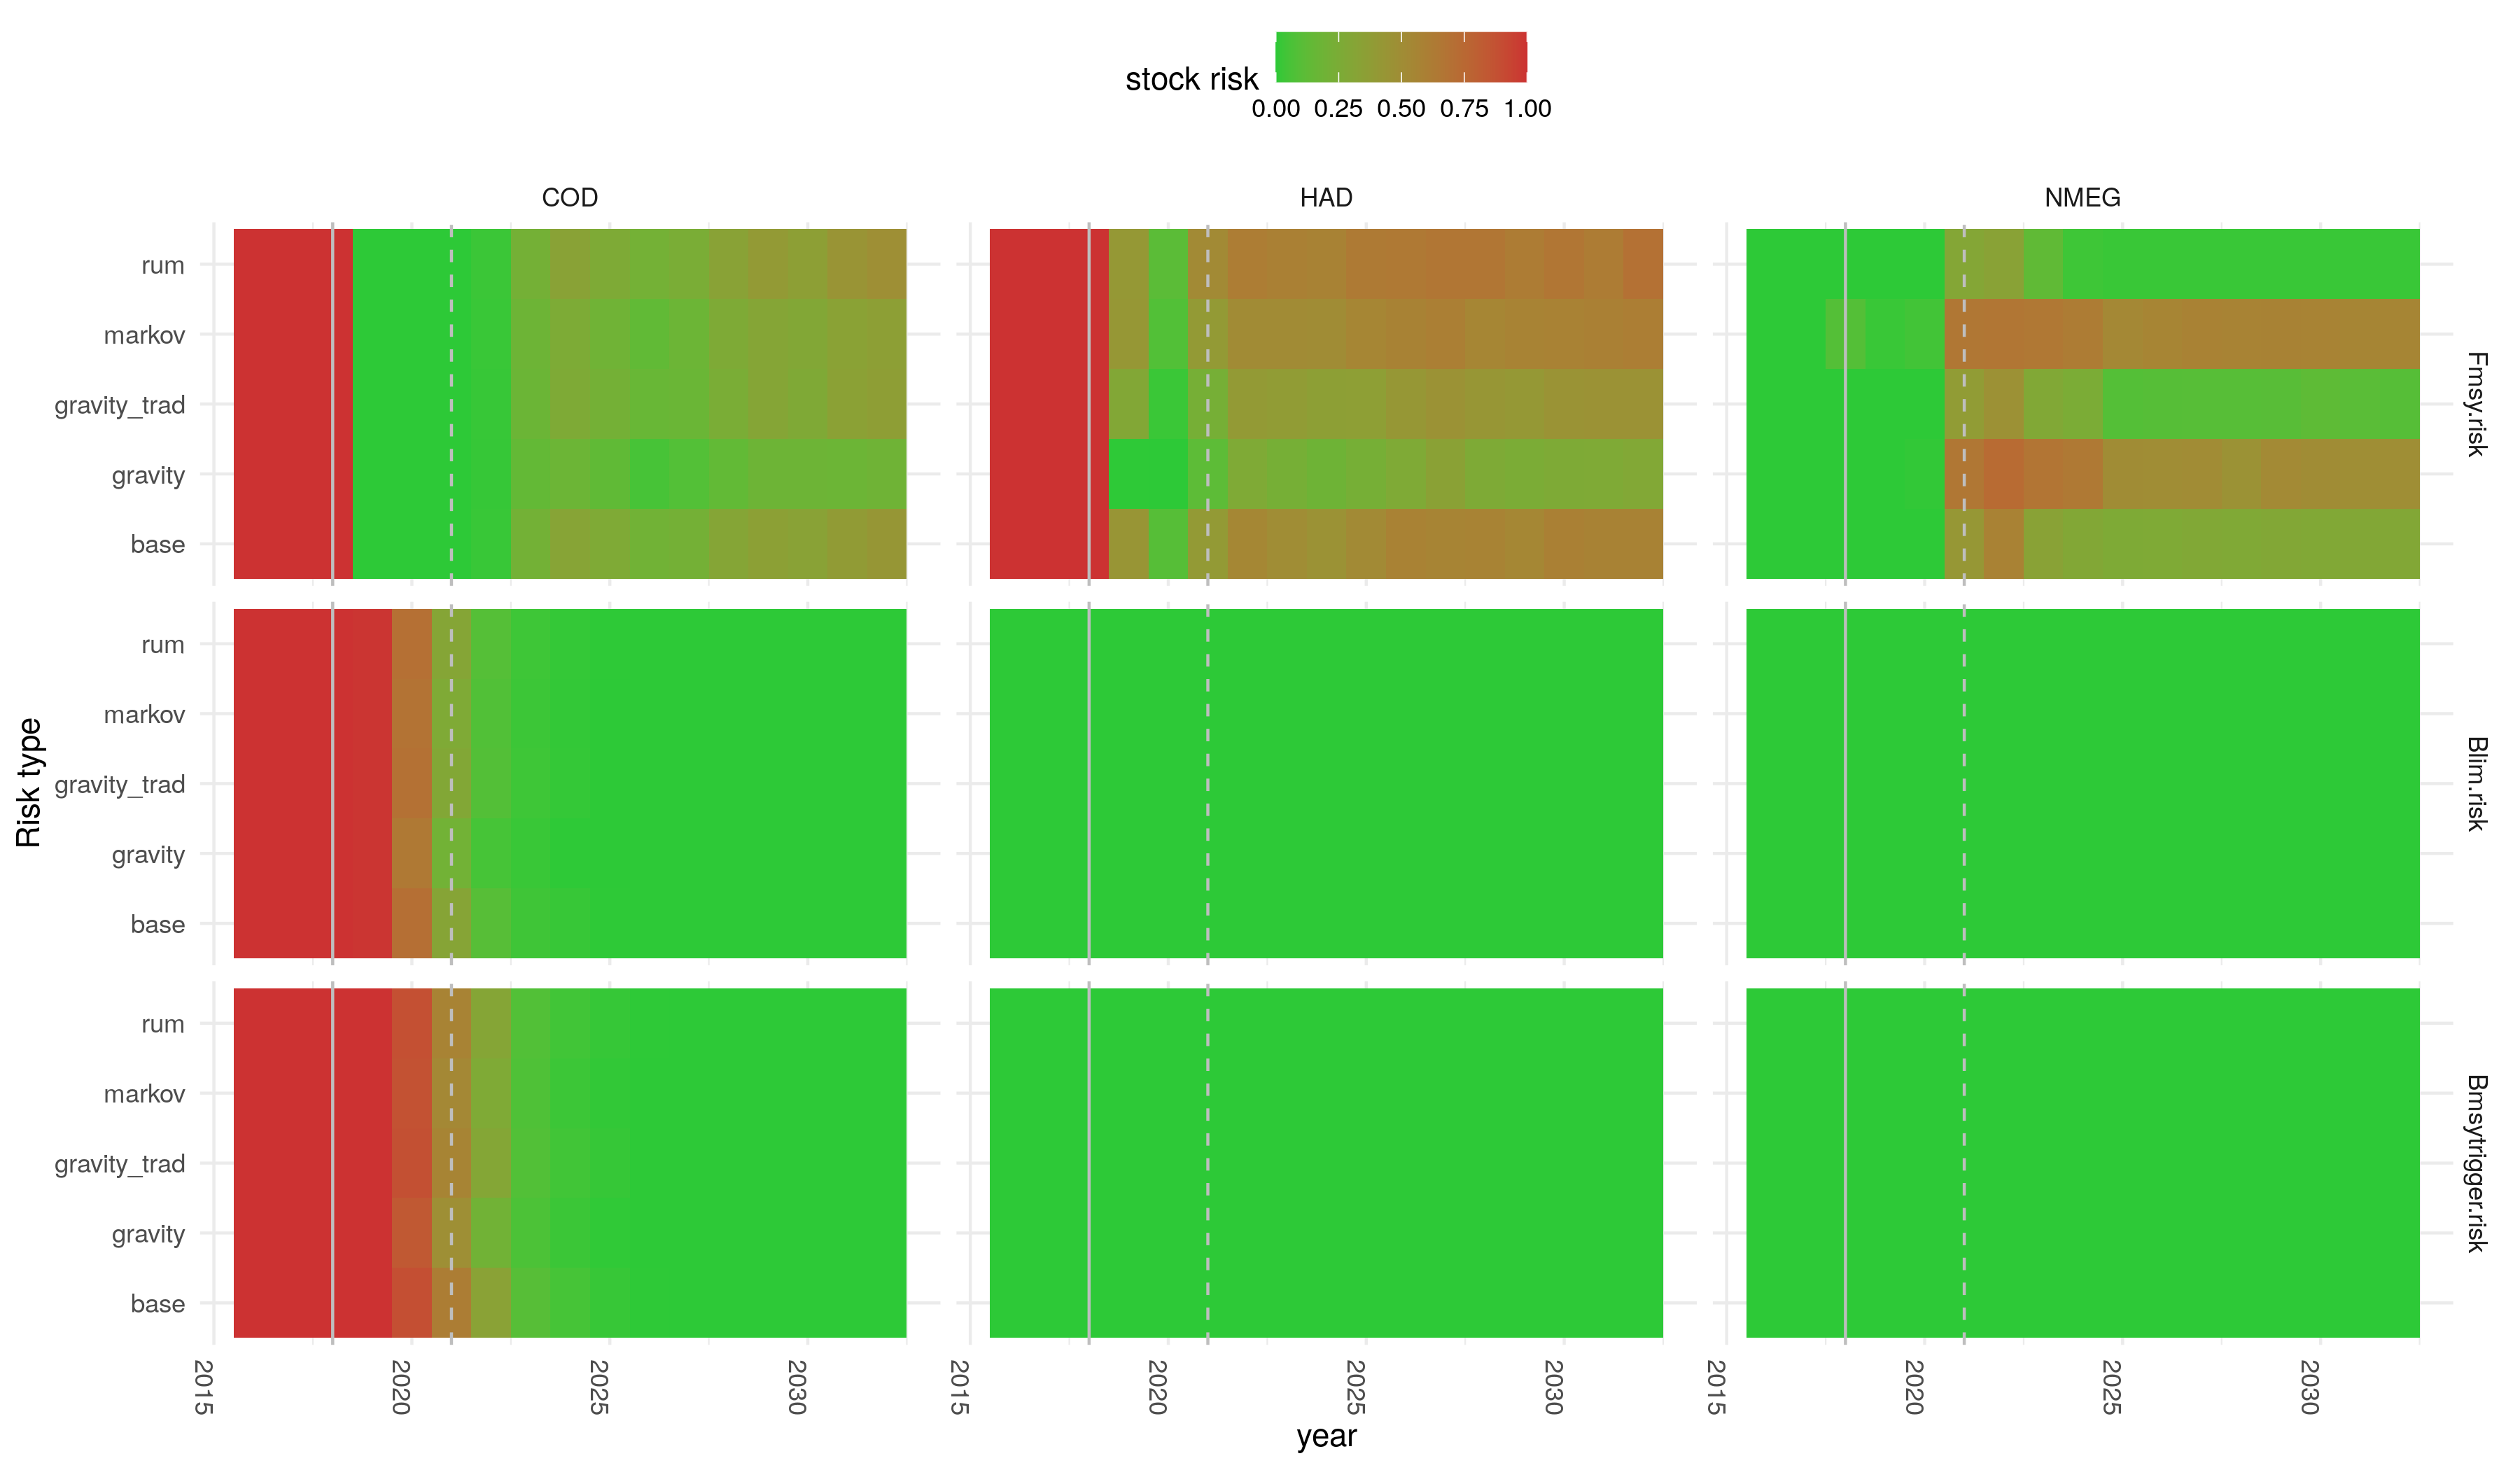
\includegraphics[width=1\linewidth]{figures/stock_risks}
	\caption{Stock risk indicators for each of the fish stock and location
		choice model scenarios. Solid
		line indicates end of the data/start of simulations and the
		dashed line the implementation of the spatial closure.} 
	\label{fig:risk}
\end{figure}	

\clearpage

\section{Appendices}

\textbf{Appendix A}

\begin{figure}[!ht]
	\centering
	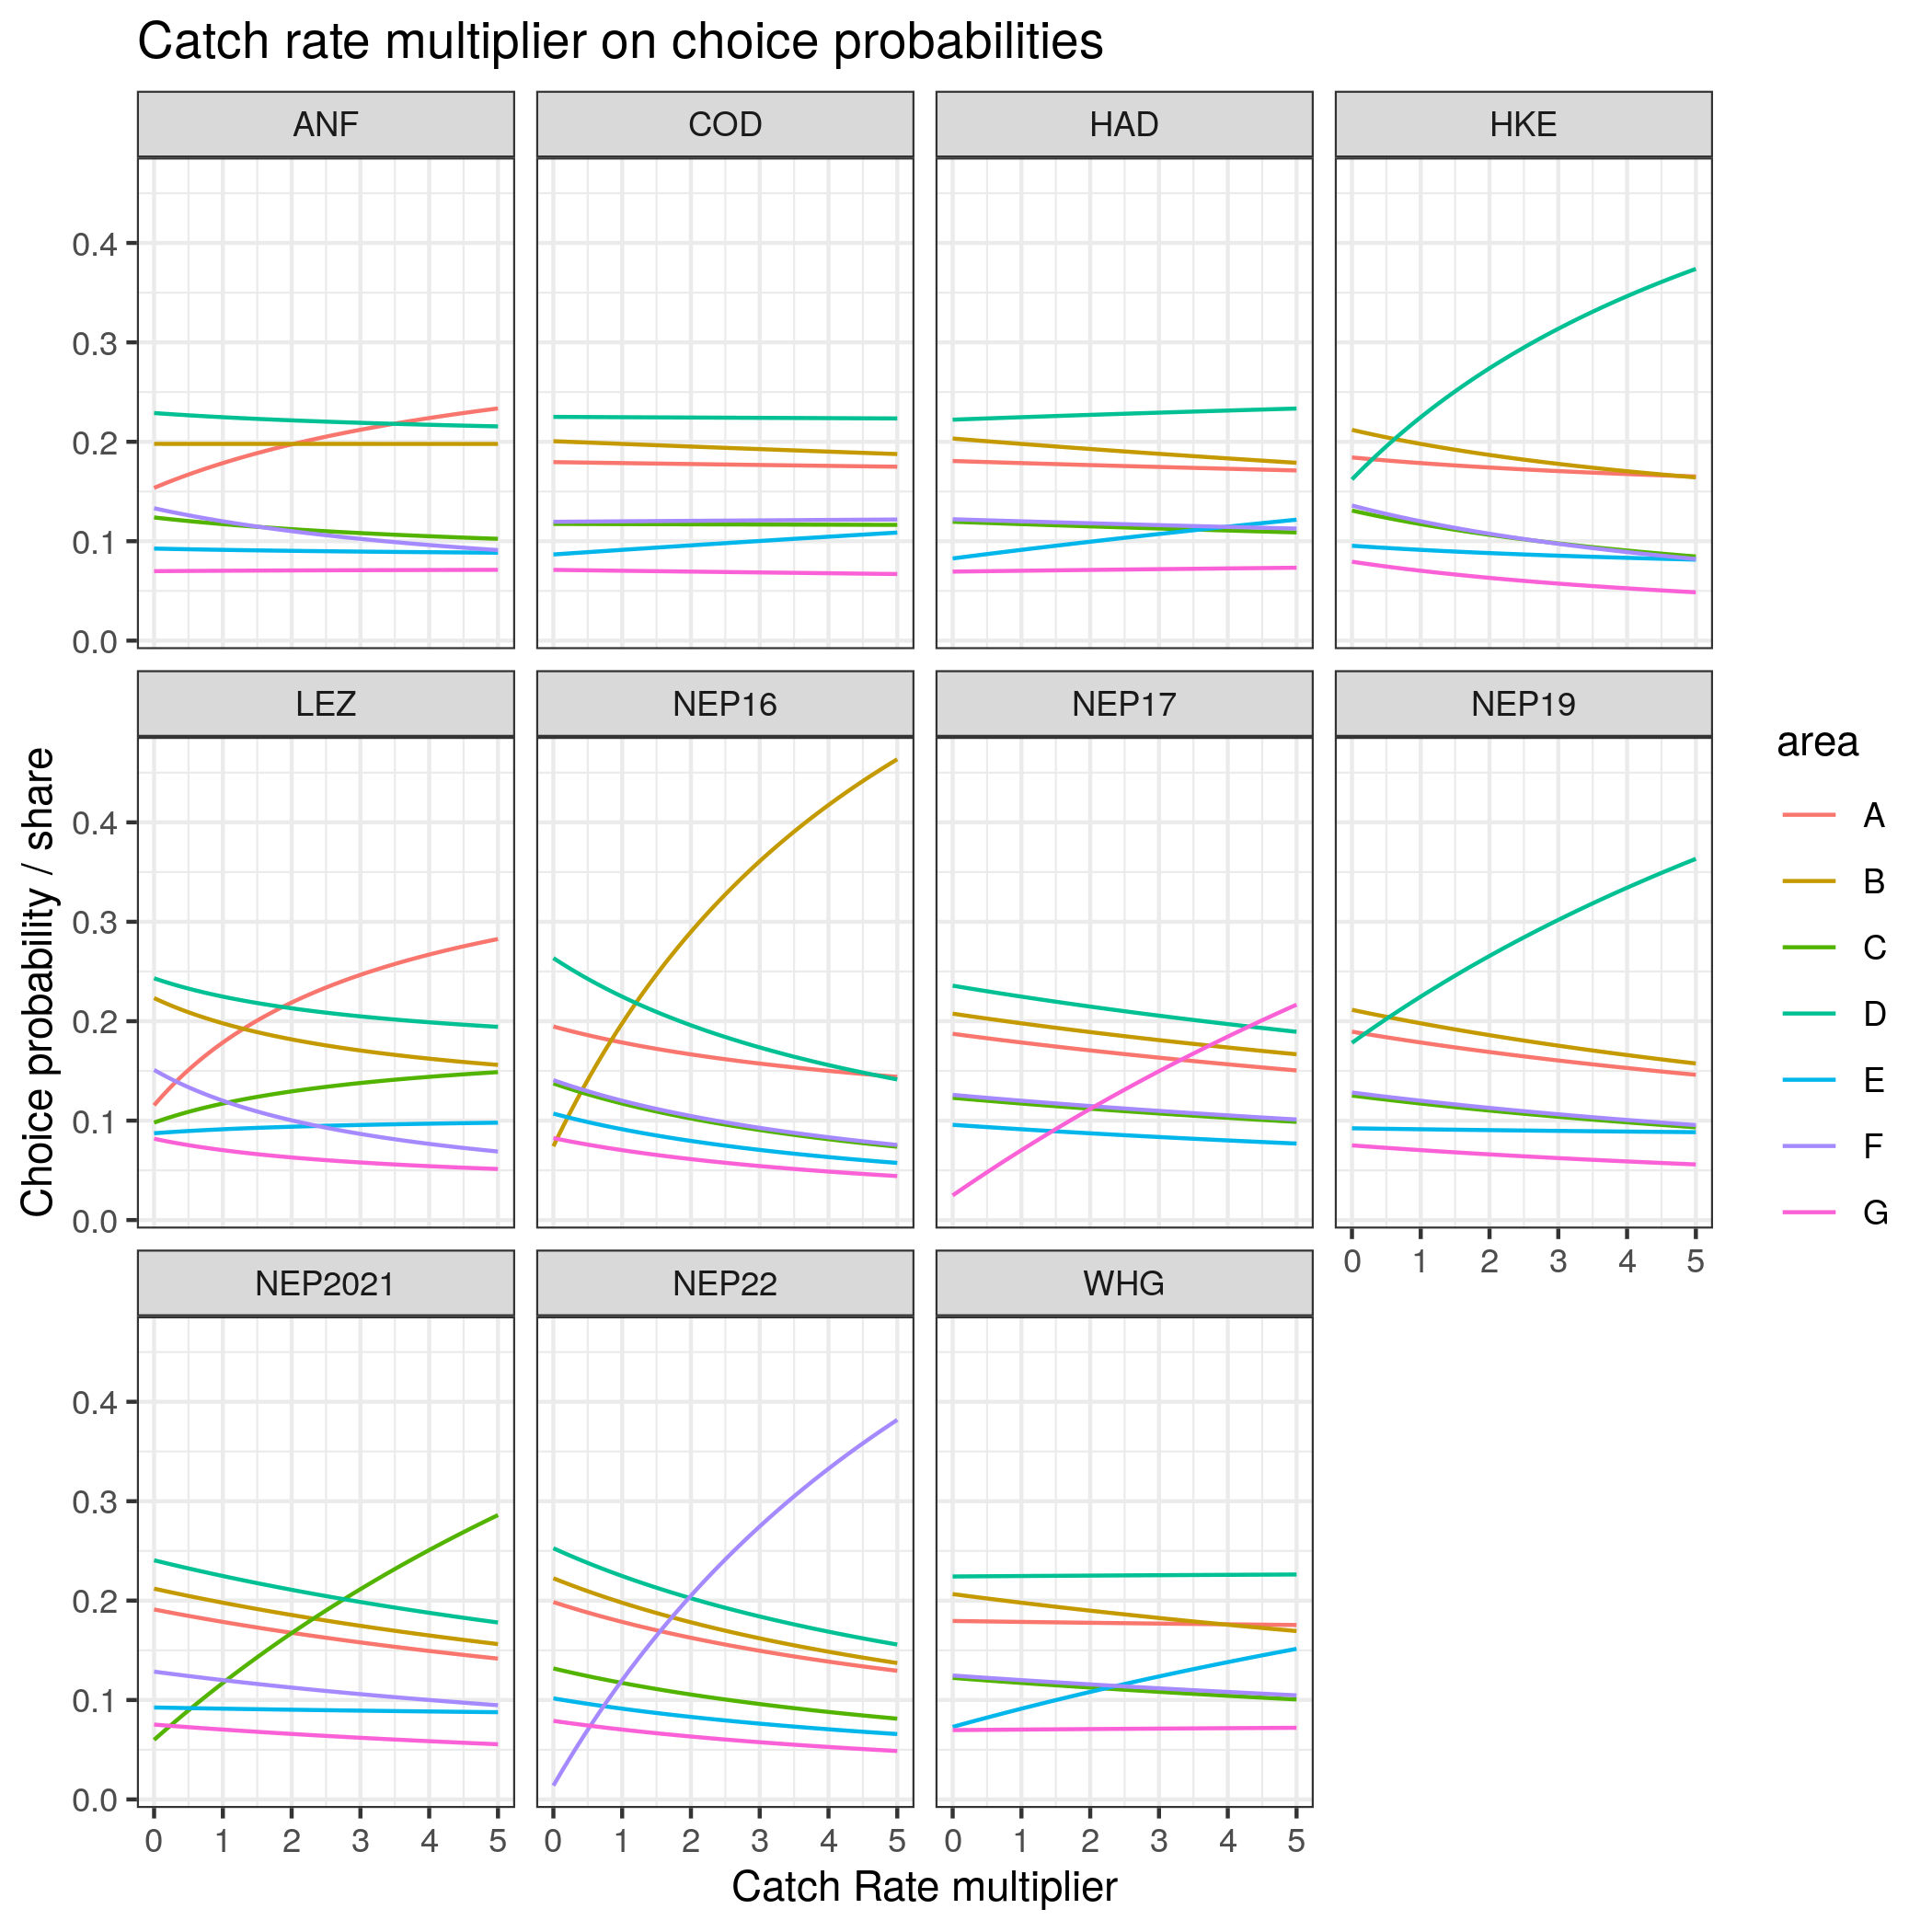
\includegraphics[width=1\linewidth]{figures/Gravity_Metier_Catch_Rate_Multiplier}
	\caption{The influence of changes in catch rates of different stocks on
	effort allocation among métier from the Gravity model.} 
	\label{fig:Grav_CR}
\end{figure}	

\begin{figure}[!ht]
	\centering
	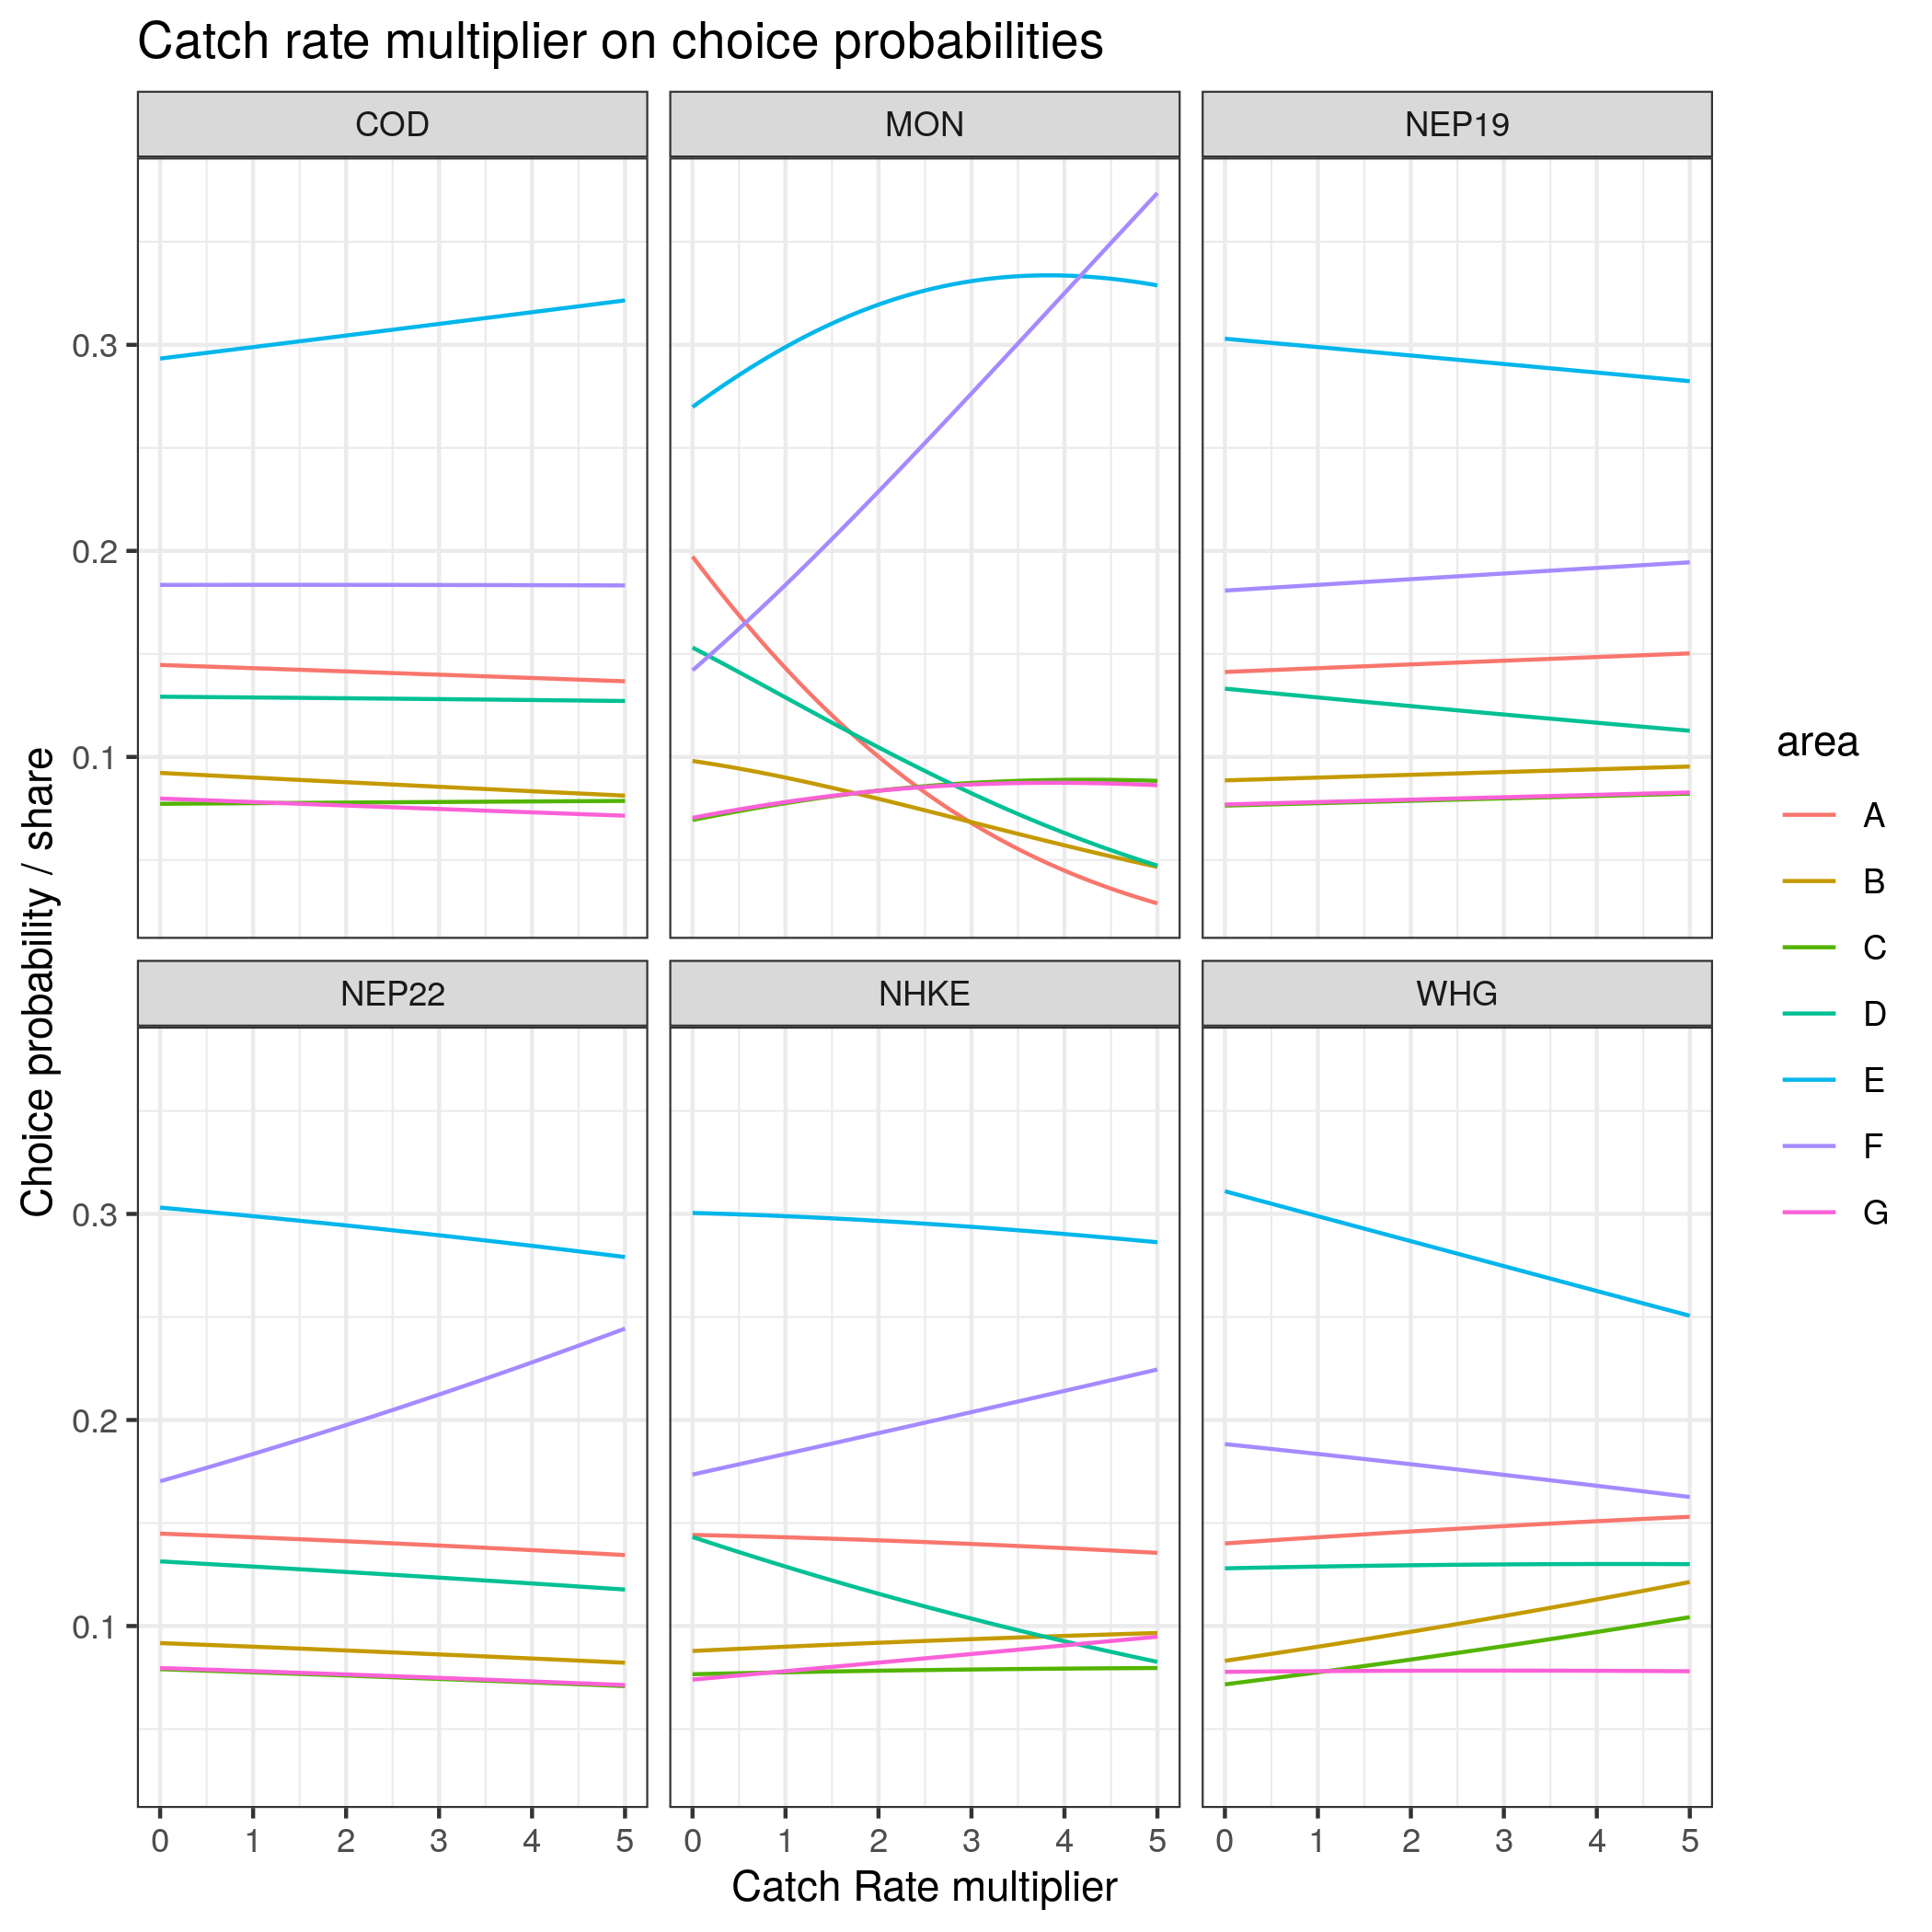
\includegraphics[width=1\linewidth]{figures/RUM_Metier_Catch_Rate_Multiplier}
	\caption{The influence of changes in catch rates of different stocks on
	effort allocation among métier from the RUM.} 
	\label{fig:RUM_CR}
\end{figure}	

\begin{figure}[!ht]
	\centering
	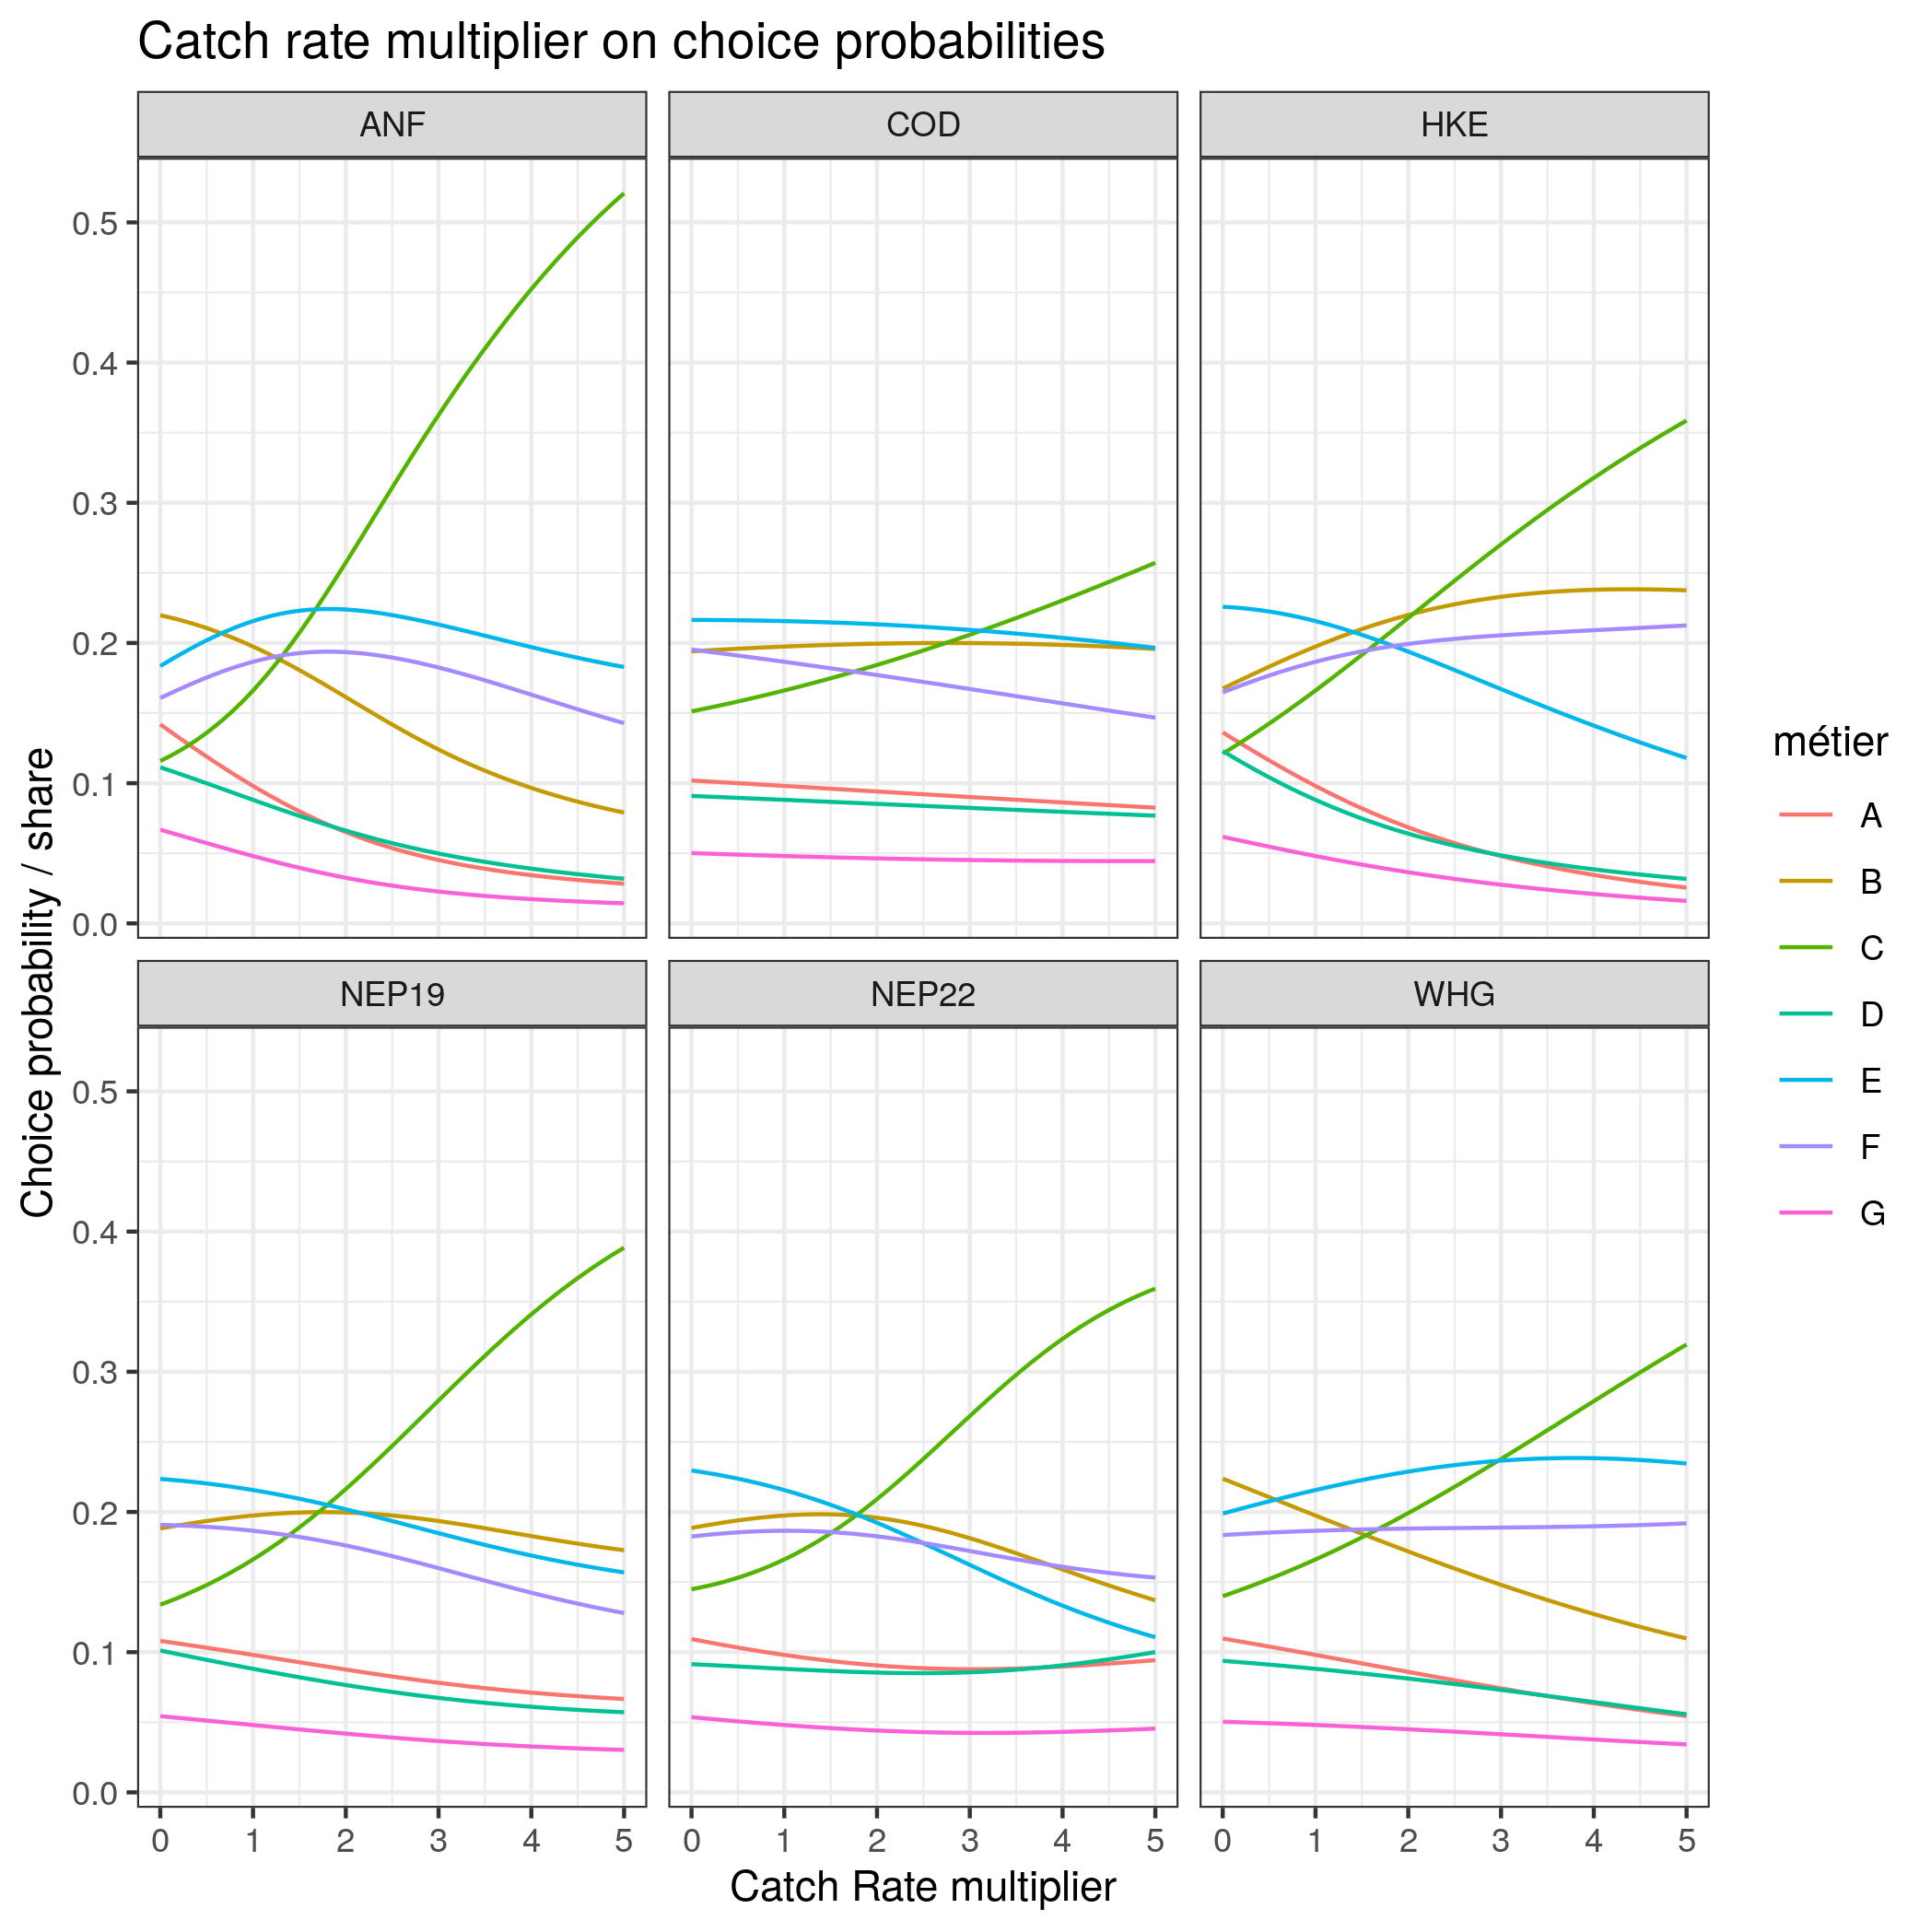
\includegraphics[width=1\linewidth]{figures/Markov_Metier_Catch_Rate_Multiplier}
	\caption{The influence of changes in catch rates of different stocks on
	effort allocation among métier from the Markov model.} 
	\label{fig:Markov_CR}
\end{figure}	

\begin{figure}[!ht]
	\centering
	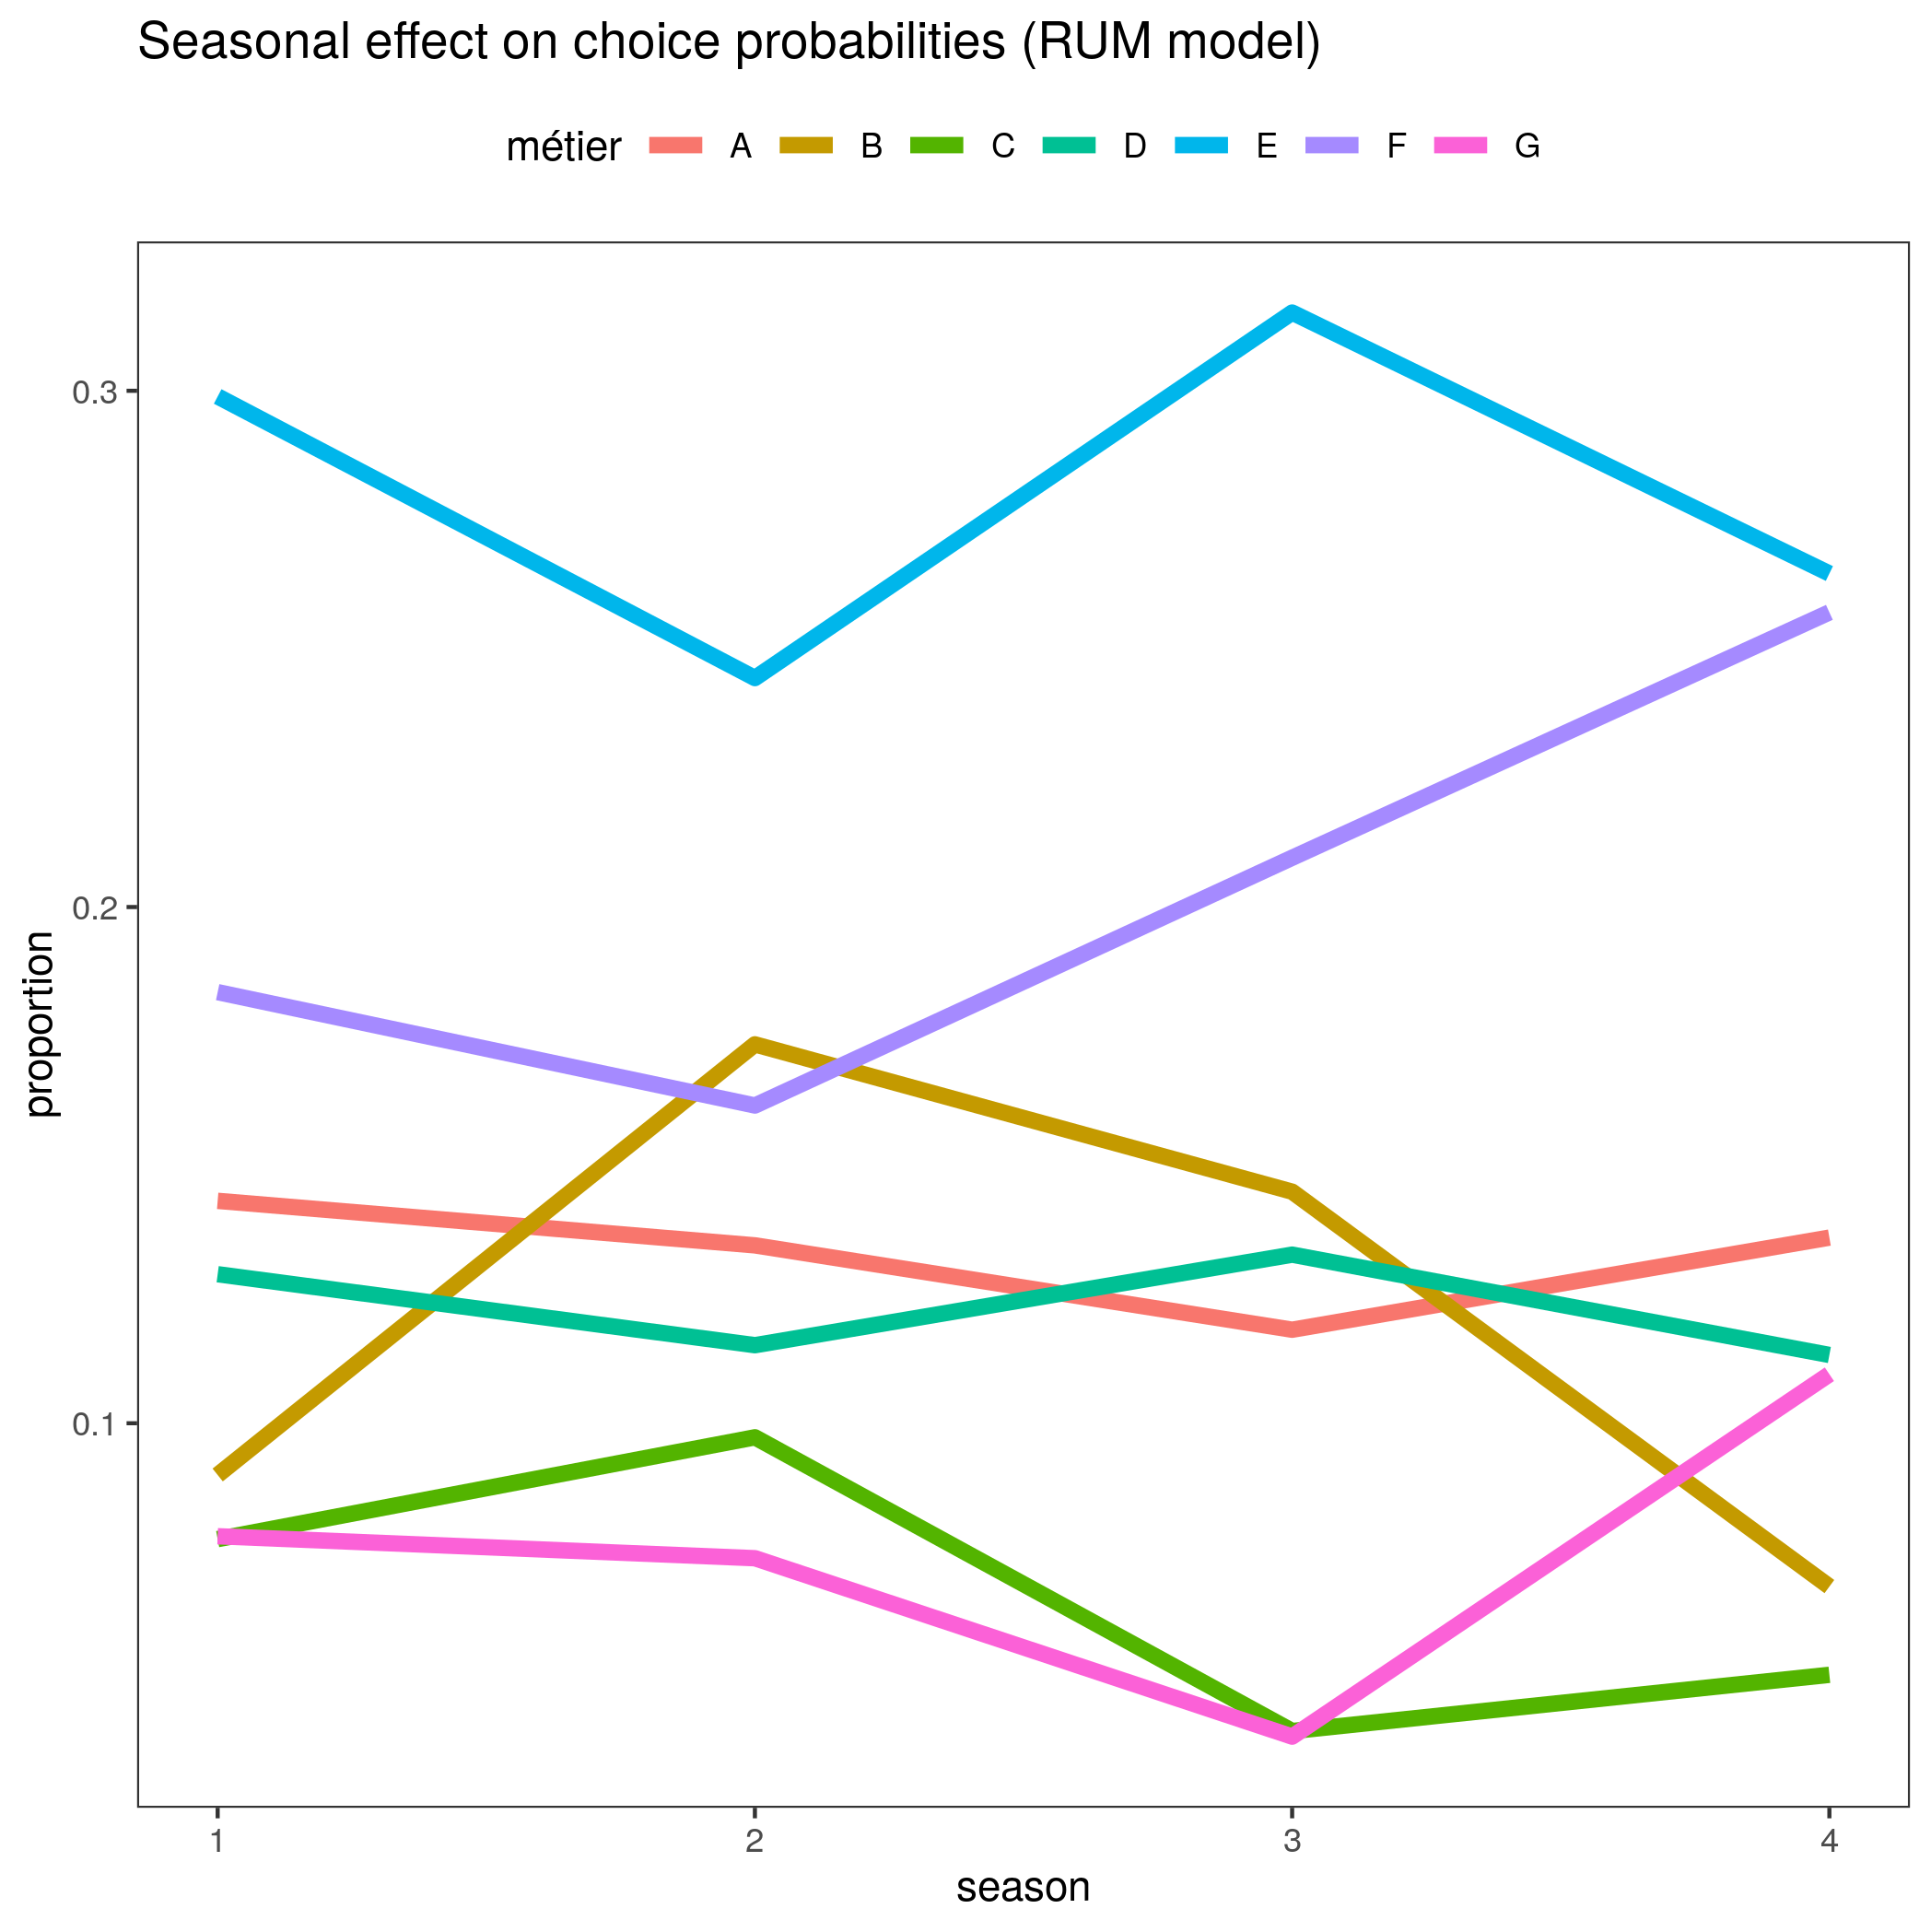
\includegraphics[width=1\linewidth]{figures/RUM_metier_seasonal_effect}
	\caption{Seasonal effect in the RUM model.} 
	\label{fig:RUM_Seas}
\end{figure}	

\begin{figure}[!ht]
	\centering
	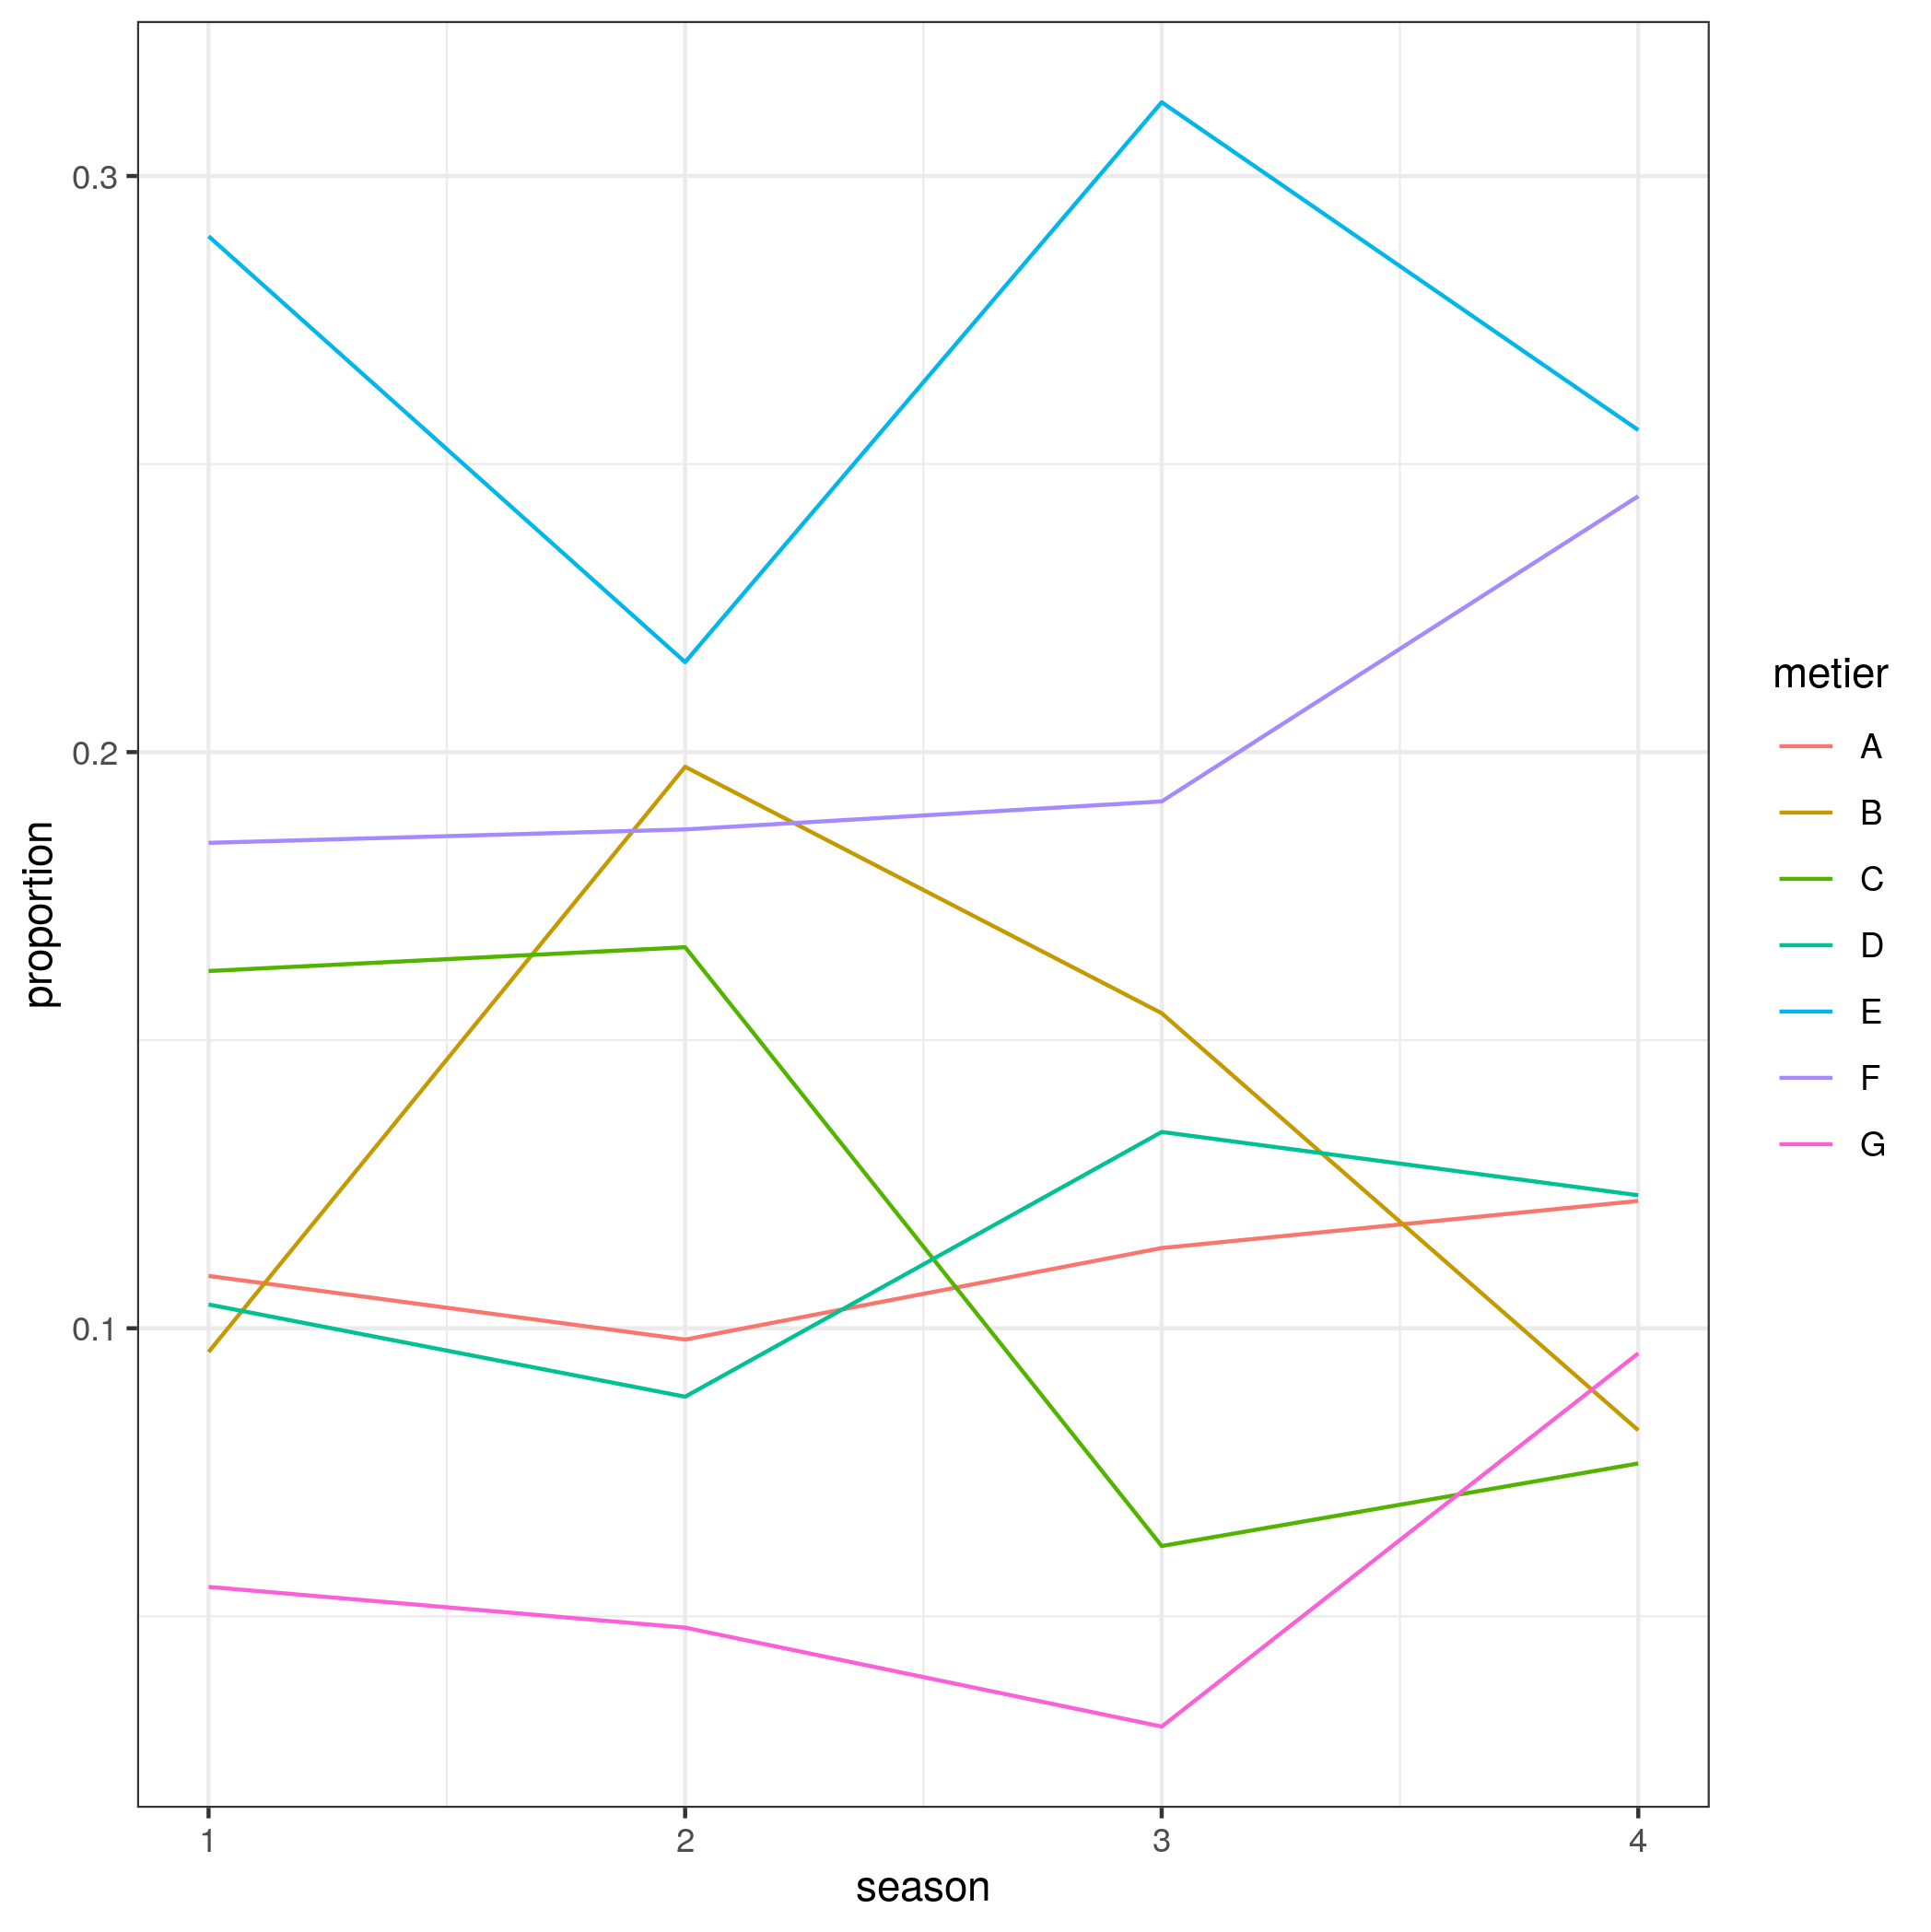
\includegraphics[width=1\linewidth]{figures/Markov_metier_seasonal_effect}
	\caption{Seasonal effect in the Markov model.} 
	\label{fig:Markov_Seas}
\end{figure}	




%%%%%%%%%%%%%%%%%%%%%%%%%
\end{document}
